\documentclass[11pt]{article}
\usepackage[margin=1in]{geometry}
\usepackage{amsmath,amssymb}
\usepackage{graphicx}
\usepackage{booktabs}
\usepackage{caption}
\usepackage{framed}
\usepackage{float}
\usepackage[section]{placeins}
\usepackage{microtype}
\usepackage[hidelinks]{hyperref}
\graphicspath{{../figures/}}
\captionsetup{font=small,labelfont=bf}
\renewcommand{\textfraction}{0.05}
\renewcommand{\topfraction}{0.95}
\renewcommand{\bottomfraction}{0.95}
\renewcommand{\floatpagefraction}{0.85}
\newcommand{\E}{\mathbb{E}}
\newcommand{\dd}{\,\mathrm{d}}

\title{Averaging Periodograms, Smoothing a Periodogram, and Multitaper Estimation Are One Estimator:\\an Intuitive Account and a Practical Recipe}
\author{Elijah Keldsen$^{1,2}$ \quad Wolfgang Ganglberger$^{3}$ \quad M.~Brandon Westover$^{2}$\\[4pt]
\small $^1$Brigham Young University, Provo, UT\\
\small $^2$Stanford University, Stanford, CA\\
\small $^3$Beth Israel Deaconess Medical Center and Harvard Medical School, Boston, MA}
\date{Draft v5 --- \today}

\begin{document}
\maketitle

\begin{abstract}
Users of multitaper spectral estimation must choose a time--bandwidth product $NW$ and a number of tapers $K$, parameters with no counterpart in the two methods everyone learns first: averaging the periodograms of segments and smoothing one periodogram across frequency. Building on an identity of Thomson (1982), we prove that the three methods are one estimator, a bank of tapers with weights built from one window by shifting it in time, shifting it in frequency, or taking orthogonal tapers. The multitaper estimate with all $N$ Slepian tapers weighted by their eigenvalues \emph{is} the periodogram averaged over a box of half-width $W$ and, in the limit of a long window, the average of periodograms of a sinc window slid along the record; the everyday estimator with $K\approx2NW-1$ tapers is that estimate with its leaky part removed. Three facts follow, quantified over 300 realizations of a spectrum spanning 65~dB. Smoothing cannot remove leakage: where the spectrum is low the untapered smoothed periodogram errs by 14~dB and the Hann-tapered one by 1.5~dB. A single taper costs a third of the degrees of freedom ($\nu=8.9$ against $14.0$), because its bank has unequal weights. And the last Slepian taper leaks: with default settings the multitaper estimate errs by 6~dB where the spectrum is low, which adaptive weights repair at the cost of half its degrees of freedom there. We give a bandwidth rule, a recipe for each route, tested code, and a demonstration on scalp EEG containing seizures, where the routes agree to a median of 1.5~dB.
\end{abstract}

\section{Introduction}

Three families of spectral estimator are in common use in electrophysiology. The first is to \emph{average periodograms}: cut the record into segments, compute the periodogram of each, and average. This is Bartlett's method \cite{bartlett1948}, with tapered and overlapping segments Welch's \cite{welch1967}, and textbooks such as Kay's \cite{kay1988} present it first, because averaging noisy estimates of the same thing plainly reduces the noise. The second is to \emph{smooth a periodogram}: convolve one periodogram of the whole record across frequency with a box (Daniell \cite{daniell1946}) or a Gaussian. This is the Blackman--Tukey estimator \cite{blackman1958}, and many pipelines apply it to spectrograms without naming it. The third is Thomson's \emph{multitaper method} \cite{thomson1982}. Two tutorials for neuroscientists \cite{babadi2014,prerau2017} have made it the recommended estimator, for good reasons: it controls leakage, it reduces variance, and it is optimal in a precise sense. Yet its two parameters have no counterpart in the first two methods: nothing in ``average the segments'' or ``smooth across frequency'' tells a user what a time--bandwidth product $NW=4$ buys, or what is lost by keeping $K=7$ tapers rather than $6$, and the tapers themselves, Slepian's discrete prolate spheroidal sequences \cite{slepian1978}, are unfamiliar objects.

\begin{figure}[!htb]
\centering
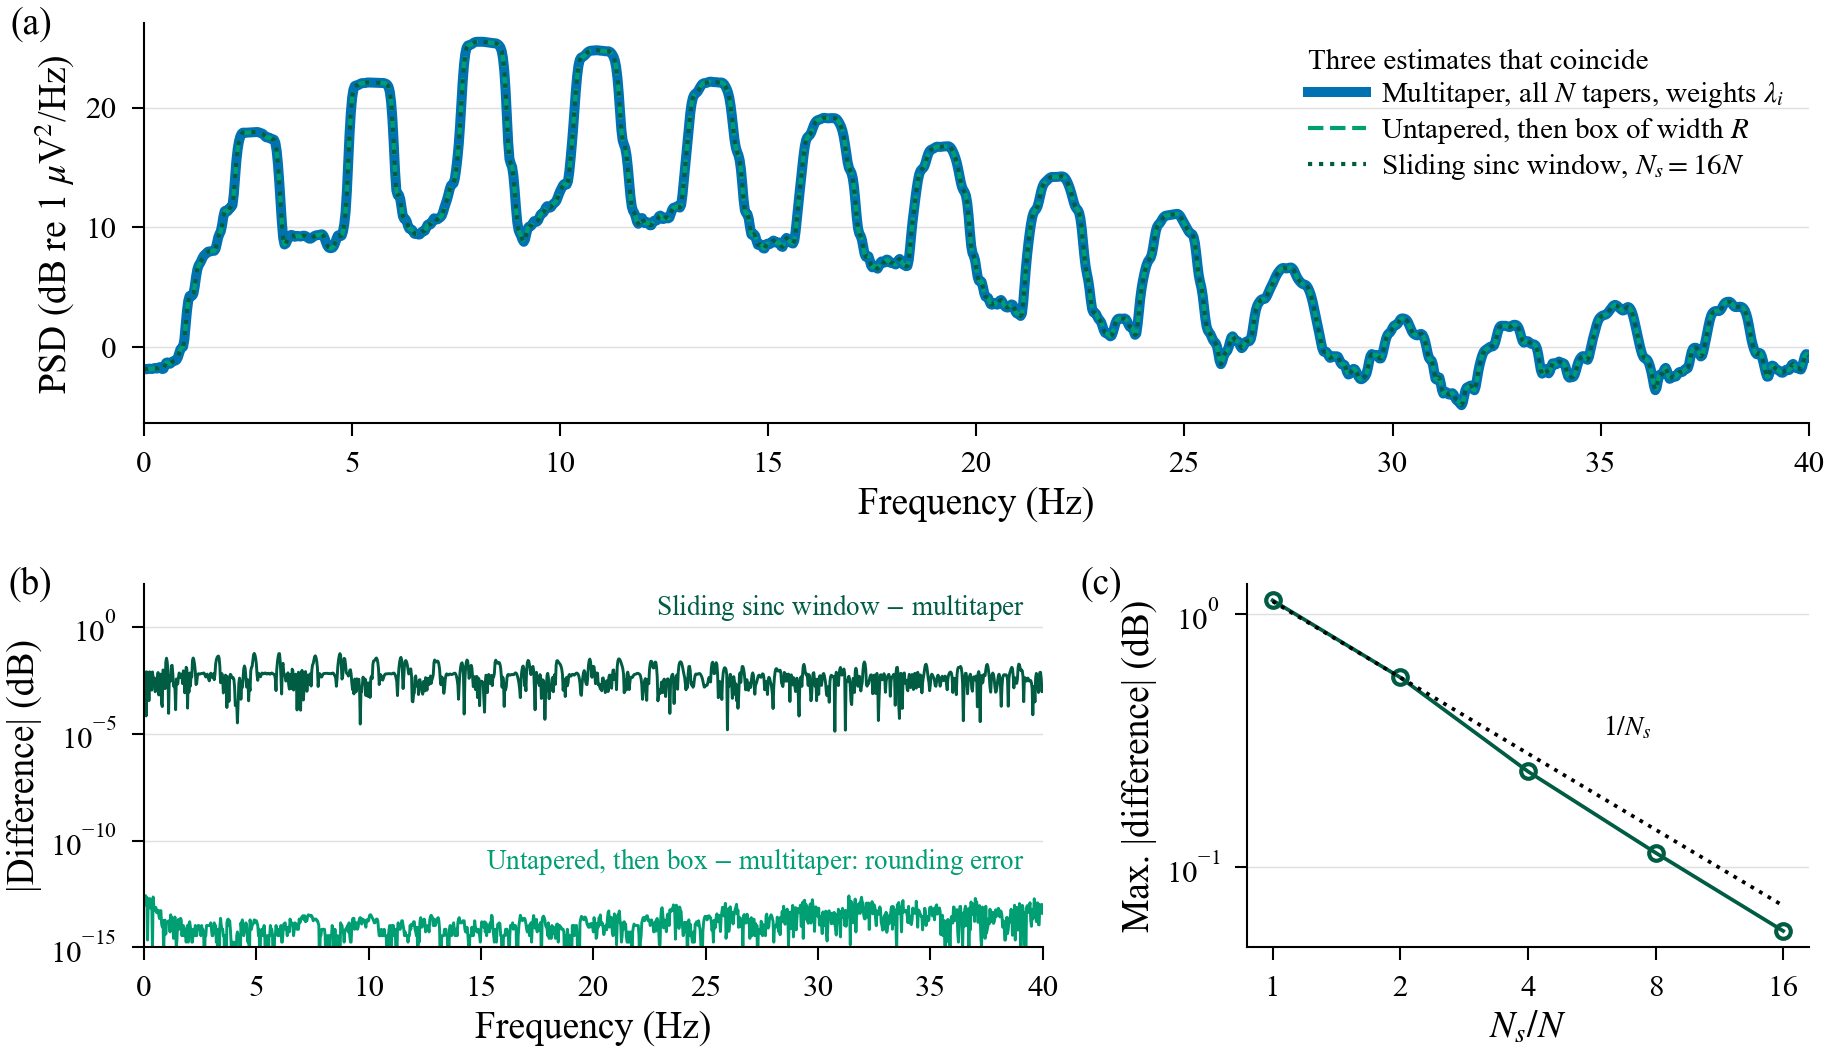
\includegraphics[width=\textwidth]{fig9_graphical_abstract.png}
\caption{\textbf{Three routes, one estimate.} (a)~Power spectral density (PSD) of eight seconds of one channel of de-identified scalp EEG at 128~Hz from the authors' archive ($N=1024$; one epoch), design half-bandwidth $W=4/N=0.5$~Hz, by three routes: the multitaper estimate with all $N$ Slepian tapers weighted by their eigenvalues $\lambda_k$ (thick grey); the untapered periodogram smoothed with a box of half-width $W$ (green); and the average of periodograms of a sinc window of half-bandwidth $W$ and length $16N$ slid across the record one sample at a time (dashed purple). (b)~Absolute differences from the multitaper estimate on a logarithmic scale: the smoothed periodogram agrees to $3\times10^{-13}$~dB, the sliding-window average to $0.06$~dB. (c)~The maximum difference of the sliding-window average versus window length, with a $1/L$ guide line. The multitaper estimate here has $\nu=17$ equivalent degrees of freedom; $\nu$ is defined in Section~\ref{sec:periodogram}.}
\label{fig:abstract}
\end{figure}

This paper shows that the three methods are one method (Fig.~\ref{fig:abstract}). All three are quadratic forms in the data, and a quadratic form is a bank of tapers with weights. Averaging periodograms builds the bank by shifting one window along the record; smoothing builds it by shifting one taper along the frequency axis; Thomson builds it from orthogonal tapers. Each bank has an expected-value kernel and an equivalent number of degrees of freedom, and once these are drawn the methods can be compared on one page. One correspondence is exact: the multitaper estimate with all $N$ Slepian tapers weighted by their eigenvalues is the periodogram averaged over a box of half-width $W$. This is equation (8.3) of Thomson's paper \cite{thomson1982}, and it appears in neither tutorial. Because averaging the periodograms of a sliding window is itself a smoothing \cite{welch1967,nuttall1982}, the same estimate is produced by sliding a sinc window across the record, and the Slepian tapers are the principal components of that sliding window.

Three things change for the user, each measured over 300 realizations of a spectrum spanning 65~dB. Leakage survives smoothing and averaging: where that spectrum is low, a box-smoothed periodogram errs by 14~dB without a taper and by 1.5~dB with one. One taper costs a third of the degrees of freedom: $\nu=8.9$ against $14.0$ at the same bandwidth, an error of 2.3 against 1.8~dB at the spectral peaks. And the default multitaper settings can lose to a tapered, smoothed periodogram, 6~dB against 1.5~dB where the spectrum is low, until adaptive weights are used; on records of 128 samples the default errs by 15~dB there.

We make five contributions. We \emph{prove} that averaging periodograms, smoothing a periodogram and multitaper estimation are one estimator, a bank of tapers with weights built three ways from one window (Section~\ref{sec:one}). We \emph{derive} the sliding-window form of Thomson's identity and \emph{identify} the Slepian sequences as the principal components of a sinc window slid across the record (Section~\ref{sec:sliding}, Appendix~\ref{app:welch}). We \emph{show} that the variance cost of the single-taper route is the slope of its eigen-weight ladder and owes nothing to Slepian sequences as such. We \emph{compute} exact kernels, leakage and degrees of freedom for ten estimators at matched bandwidth, and their errors over an ensemble (Tables~\ref{tab:dof} and \ref{tab:ensemble}). And we \emph{present} a recipe for each route, \emph{explain} how to choose its bandwidth from the narrowest feature that matters (Section~\ref{sec:howwide}), and \emph{test} it on scalp EEG containing focal seizures (Section~\ref{sec:eeg}).

The method throughout is one: write each estimator as a quadratic form, diagonalize it, and compare through its kernel and its ladder. Sections~\ref{sec:periodogram} and \ref{sec:fixes} set up the kernel picture and the three classical ways of shaping it; Section~\ref{sec:mt} presents multitaper estimation as usual; Section~\ref{sec:one} shows that the three are one and what their everyday versions trade; Sections~\ref{sec:recipe} and \ref{sec:eeg} give the recipe and the EEG demonstration. Proofs are in the appendices.

\section{The periodogram, and the one picture that explains it}
\label{sec:periodogram}

Every estimator in this paper is the true spectrum blurred by a kernel, plus noise, and the periodogram is the case in which the kernel is Fej\'er's and the noise is worst. Let $x_0,\dots,x_{N-1}$ be $N$ samples of a stationary signal, with the sampling interval as the unit of time so that frequency $f$ is in cycles per sample and runs from $-\tfrac12$ to $\tfrac12$. The periodogram is
\begin{equation}
\hat I(f) = \frac{1}{N}\Bigl|\sum_{t=0}^{N-1} x_t\, e^{-i2\pi f t}\Bigr|^2 ,
\label{eq:periodogram}
\end{equation}
the squared magnitude of the discrete Fourier transform, evaluated on as fine a grid as one likes by zero-padding with the fast Fourier transform (FFT). It has two well-known defects, both visible in Fig.~\ref{fig:motif}(a,\,e).

\begin{figure}[!htb]
\centering
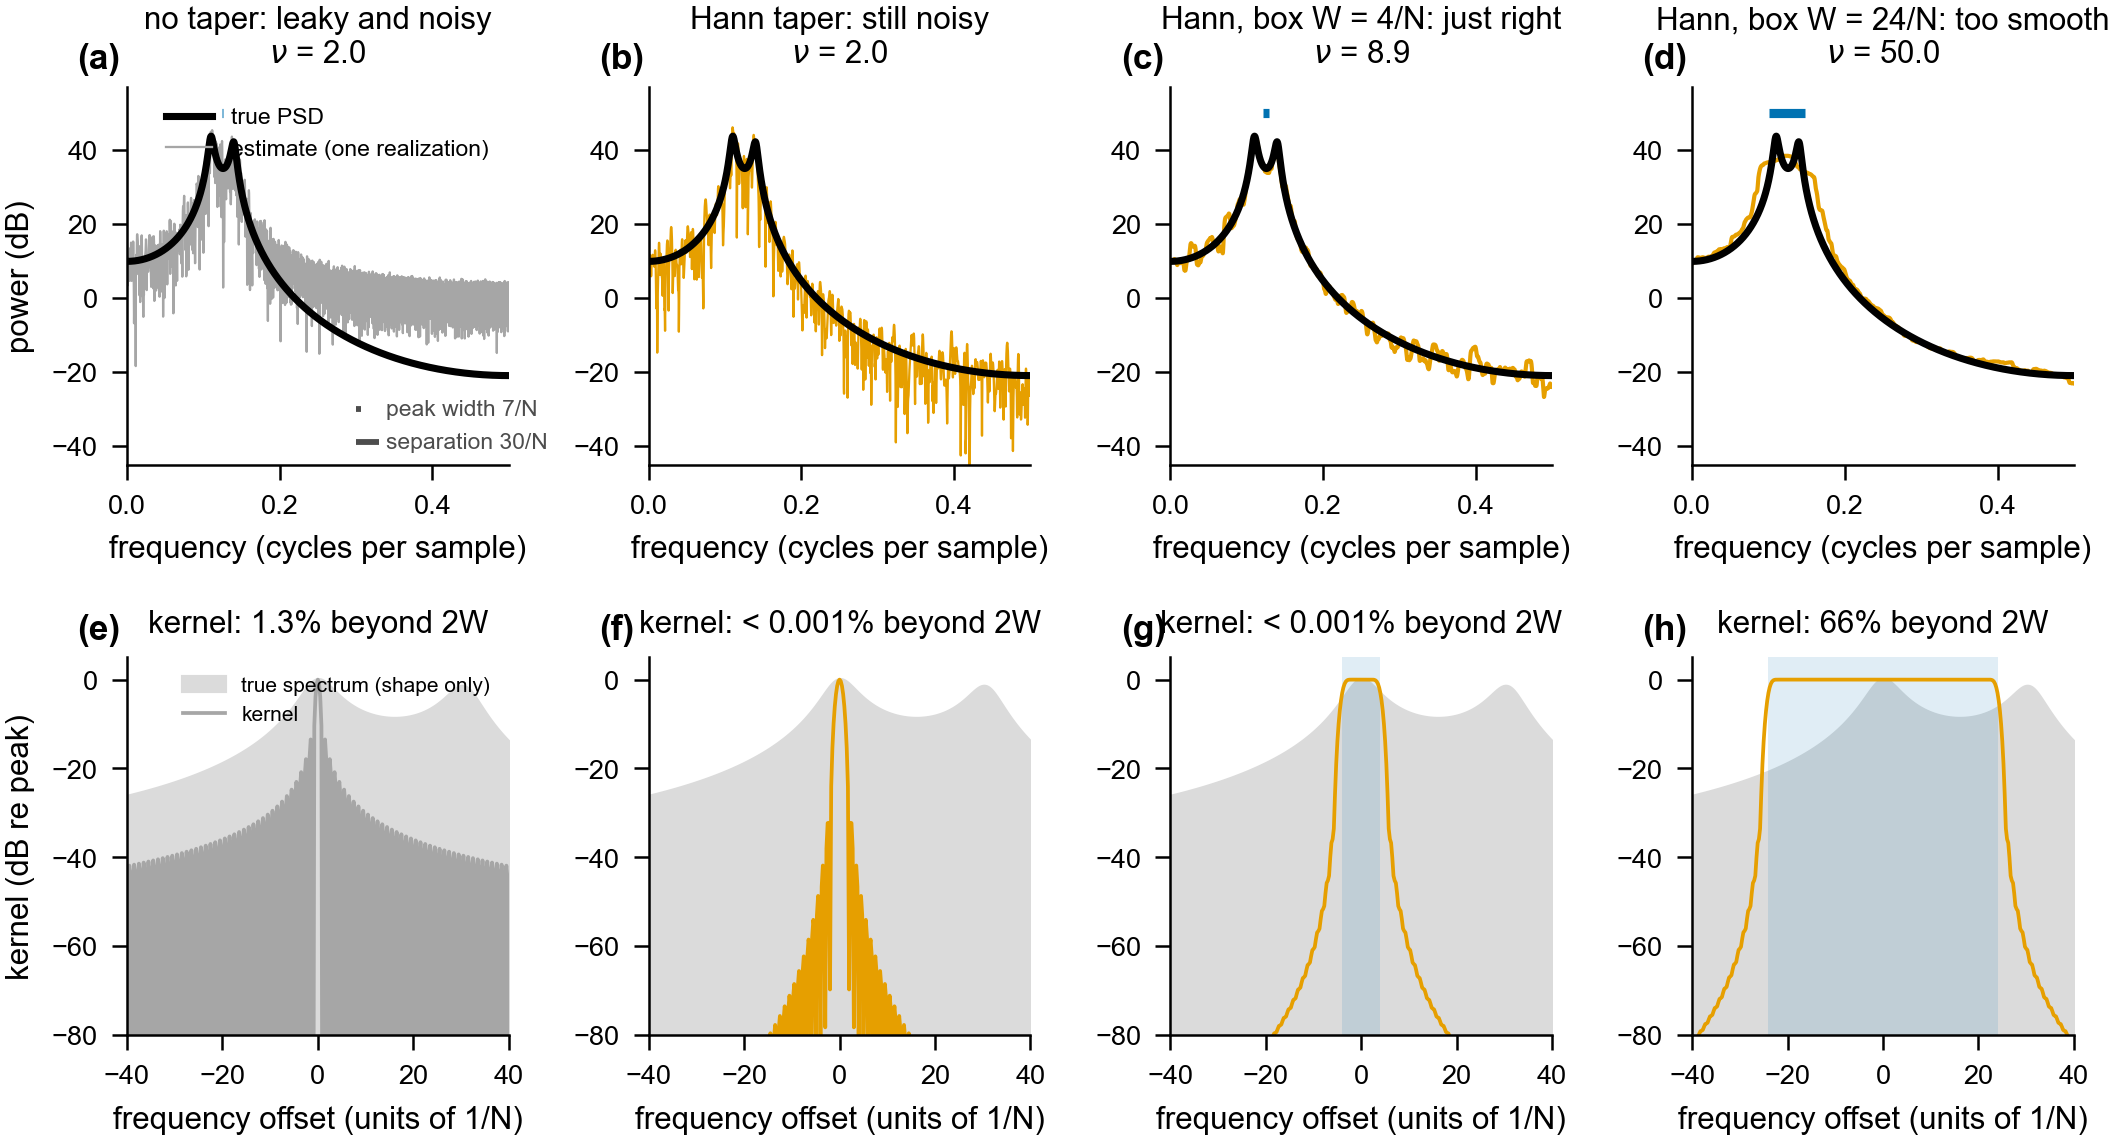
\includegraphics[width=\textwidth]{fig0b_estimates_kernels.png}
\caption{\textbf{Every estimator is the true spectrum blurred by a kernel, plus noise.} (a--d)~One realization ($N=1024$) of an autoregressive process whose PSD (black) has two peaks $7/N$ wide at half power and $30/N$ apart on a background spanning 65~dB, estimated by the periodogram (a), a Hann-tapered periodogram (b), the same smoothed with a box of half-width $W=4/N$, for which $2W$ equals the width of a peak (c), and smoothed with $W=24/N$, for which $2W$ exceeds the separation of the peaks (d). The short blue bar above the peaks is the half-power width of each estimator's kernel; the grey bars in (a) mark the peak width and separation; $\nu$ is the equivalent degrees of freedom. (e--h)~Each estimator's expected-value kernel in dB relative to its peak, drawn over the true spectrum around its peaks (grey; only its shape matters, not its level); blue shading marks $|f|\le W$; ``beyond $2W$'' is the fraction of the kernel's power outside $|f|\le 2W$, our measure of broadband leakage. Reading across: the Fej\'er kernel's slow skirts leak power from the peaks into the region 40~dB below them (a,\,e); the Hann taper lowers the skirts by 20 to 50~dB at the price of a main lobe twice as wide (f); a box as wide as a peak is just right (g); a wider one merges the peaks (h).}
\label{fig:motif}
\end{figure}

\paragraph{It is noisy.} At any one frequency the periodogram of a Gaussian signal is distributed like the true power spectral density (PSD) times a chi-square variable with two degrees of freedom divided by two. Its standard deviation equals its mean, and recording for longer does not help: a longer record gives more frequency points, each just as noisy.

\paragraph{It leaks.} Its expected value is the true PSD $S$ convolved with a kernel,
\begin{equation}
\E[\hat I(f)] = \int_{-1/2}^{1/2} F(f-f')\,S(f')\dd f' ,
\qquad F(f)=\frac{1}{N}\biggl(\frac{\sin N\pi f}{\sin \pi f}\biggr)^{2},
\label{eq:fejer}
\end{equation}
where $F$ is Fej\'er's kernel, the squared Fourier transform of the rectangular window that truncated the record. $F$ has a main lobe of width about $2/N$ and side lobes that fall off only as $1/f^2$. Where the true spectrum varies by tens of decibels across the band, as neural spectra do, the tails of $F$ carry power from the strong region into the weak one, and the estimate floors at a level set by leakage rather than by the signal.

\paragraph{The one picture.} Equation~\eqref{eq:fejer} is the template for everything that follows. Every estimator in this paper satisfies
\begin{equation}
\E[\hat S(f)] = \int H(f-f')\,S(f')\dd f' ,
\label{eq:kernel}
\end{equation}
a blurred view of the truth through an \emph{expected-value kernel} $H$, plus noise around that expected value. Three numbers characterize an estimator: the width of the main lobe of $H$ (\emph{resolution}), the height of its skirts (\emph{leakage}), and the noise, reported as an equivalent number of degrees of freedom $\nu$ (\emph{variance}: the estimate behaves like $S\,\chi^2_\nu/\nu$, with relative standard error $\sqrt{2/\nu}$, about $4.3\sqrt{2/\nu}$~dB, and an approximate 95\% confidence interval from $\nu\hat S/\chi^2_{\nu,0.975}$ to $\nu\hat S/\chi^2_{\nu,0.025}$). The periodogram has the narrowest possible main lobe, bad leakage, and $\nu=2$. Every improvement trades among the three. Appendix~\ref{app:quadratic} gives the formulas from which the kernel and $\nu$ of any estimator in this family are computed exactly; all numbers below come from them.

\section{Three classical fixes, seen as kernel design}
\label{sec:fixes}

\subsection{Average periodograms of segments}
\label{sec:averaging}
Bartlett's remedy \cite{bartlett1948} for the noise is to cut the record into $M$ segments of length $L$, compute a periodogram of each, and average. Non-overlapping segments give independent estimates with $\nu=2$ each, so the average has $\nu\approx2M$. The price is resolution: each segment's kernel is the Fej\'er kernel of length $L$, with a main lobe of width $2/L=2M/N$, and averaging does not narrow it. Welch \cite{welch1967} tapers each segment to control leakage and overlaps segments by half their length to recover the data lost at the tapered ends; Hann segments at 50\% overlap are nearly uncorrelated \cite{welch1967,percival1993}, so $\nu$ is again close to twice their number (13.4 for seven segments in Table~\ref{tab:dof}). In the kernel picture the estimator's kernel is the segment taper's own spectral window $|\mathcal{W}_L(f)|^2$, whatever the overlap, and the segment length is the bandwidth: more, shorter segments give more $\nu$ and a wider kernel.

\subsection{Smooth one periodogram}
\label{sec:smoothing}
The second remedy keeps one periodogram of the whole record and averages it over a window of frequencies: a box of half-width $W$ \cite{daniell1946}, a Gaussian, or any non-negative kernel $G$. Expectation commutes with averaging, so the kernel of the smoothed estimate is the kernel of the unsmoothed one convolved with the smoothing window, $H=G*F$. The main lobe widens to about $2W$, which is now the resolution and is under direct control. The noise drops: periodogram values spaced $1/N$ apart are nearly independent, so a band of width $2W$ pools roughly $2NW$ of them and $\nu\approx2\cdot2NW$. And the leakage is unchanged, because convolving with a non-negative window spreads the skirts around but cannot cancel them. This is the Blackman--Tukey estimator \cite{blackman1958} computed in the frequency domain, and it is what a pipeline does when it convolves a spectrogram with a Gaussian along frequency. Section~\ref{sec:sliding} shows that this remedy and the previous one are the same.

\subsection{Taper first: shaping the skirts}
\label{sec:tapering}
Neither averaging nor smoothing does anything about leakage, and both are commonly applied to tapered periodograms for that reason. Multiply the data by a window $w_t$ that goes smoothly to zero at both ends before transforming; the kernel becomes $|\mathcal{W}(f)|^2$, the squared transform of the taper. For the Hann window the first side lobe drops from $-13$ to $-31$~dB and the tails fall as $1/f^6$ instead of $1/f^2$; the price is a main lobe twice as wide (Fig.~\ref{fig:motif}f). Tapering does nothing for the variance: a single tapered periodogram still has $\nu=2$ (Fig.~\ref{fig:motif}b). The two operations are complementary: the taper decides how fast the skirts fall, the smoothing window or segment length decides how wide the top is.

\subsection{How wide? Blur against noise}
\label{sec:howwide}
Bandwidth trades blur against noise. Whichever remedy is used, a bandwidth must be chosen: the segment length, the half-width $W$, or, in Section~\ref{sec:mt}, the time--bandwidth product. Fig.~\ref{fig:sweep} shows the choice for smoothing. Widening the box pools more periodogram ordinates, so the noise falls as $4.3\sqrt{2/\nu}$~dB with $\nu$ roughly proportional to $NW$ (blue). It also blurs the spectrum over a width $2W$, so a peak narrower than $2W$ is lowered and broadened and a valley narrower than $2W$ is filled in; this bias is zero for a flat spectrum and grows with the curvature of $S$ on the scale of the box (orange). The two add in quadrature and the total has a broad minimum where they are comparable.

What fixes the position of that minimum is the narrowest feature that has to survive. The peaks in Fig.~\ref{fig:motif} are $7/N$ wide, so a box with $2W\approx7/N$, that is $W=4/N$, is as wide as it can be without flattening them: the estimate follows the truth to within its own $\pm2$~dB noise with $\nu=8.9$. A narrower box leaves noise on the table ($\nu=2$, error 6~dB); a box wider than the separation of the peaks averages them into one ($W=24/N$, $\nu=50$), and its error over the peak region is again 6~dB even though the estimate looks clean. The optimum depends on what is scored, $W\approx8/N$ over the whole band, most of which is featureless, and $W\approx4$--$5/N$ over the peaks, so it cannot be known in advance for real data. The practical rule is the one the figure illustrates: decide which feature is the narrowest one that matters, an alpha peak one to two hertz wide, say, and set $2W$ to about its width. Data-driven choices exist for smoothed periodograms \cite{wahba1980,hurvich1985} and for multitaper estimates \cite{haley2017}; they optimize a whole-band criterion and are subject to the same caveat.

\begin{figure}[!htb]
\centering
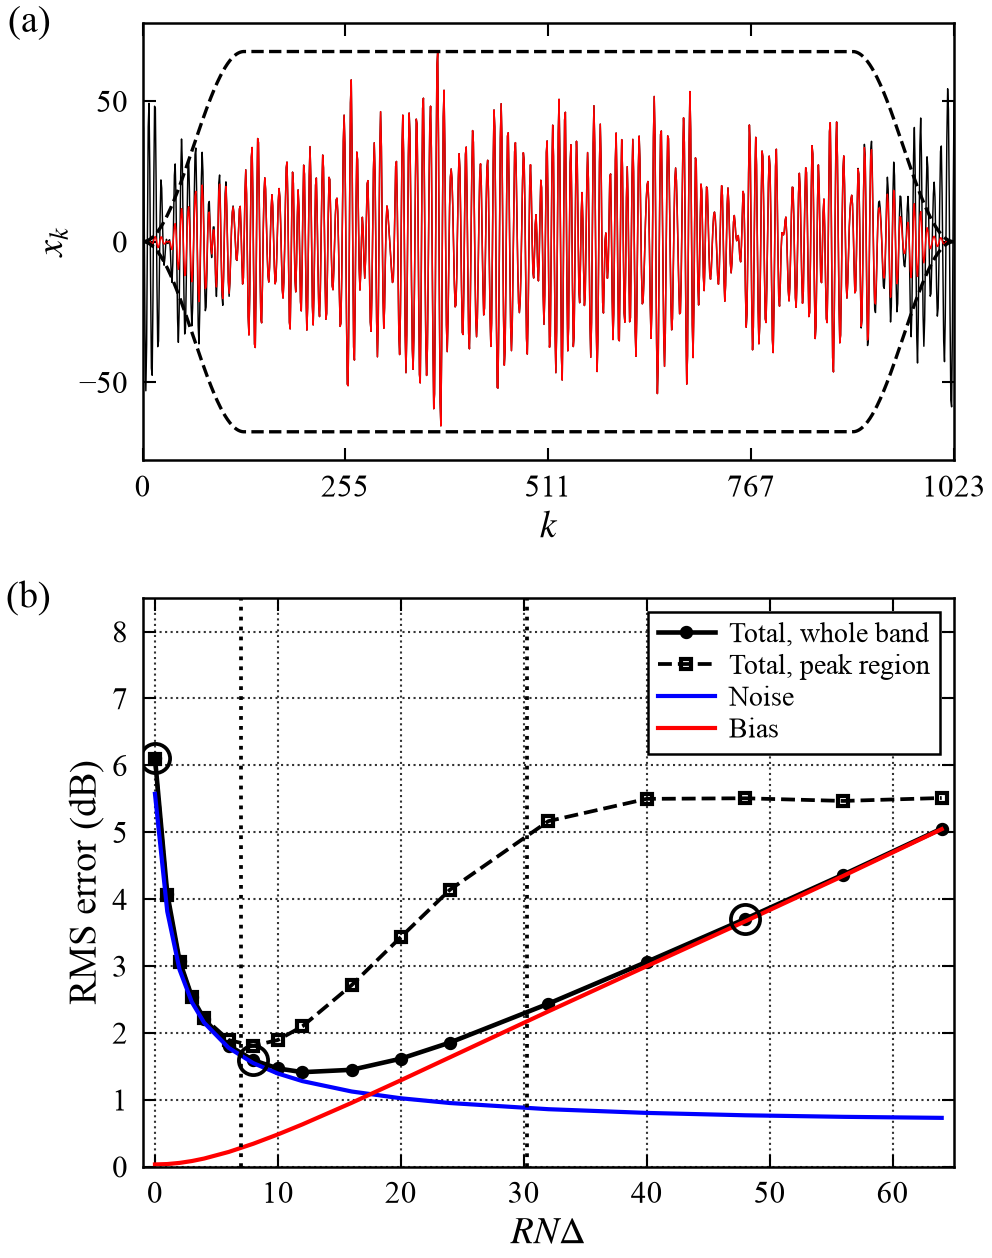
\includegraphics[width=\textwidth]{fig0a_record_sweep.png}
\caption{\textbf{Choosing the bandwidth.} (a)~The record of Fig.~\ref{fig:motif}: $N=1024$ samples of the AR(4) process (grey), the Hann taper scaled to the record's peak amplitude (dashed), and the tapered record (orange). (b)~Root-mean-square error over frequency, in dB, of the Hann-tapered, box-smoothed estimate against the true PSD as the box half-width varies, averaged over 300 independent realizations; no error bars are shown because the curves are ensemble averages. Noise (the standard deviation of the estimate, blue) falls with $W$, blur (the bias of the kernel, orange) grows, and their total (black) has a broad minimum that sits at smaller $W$ when only the peak region, $0.09$ to $0.16$ cycles per sample, is scored (dashed). The circled points are panels (b), (c) and (d) of Fig.~\ref{fig:motif}.}
\label{fig:sweep}
\end{figure}

\section{Multitaper estimation, as usually presented}
\label{sec:mt}

Thomson's method \cite{thomson1982} buys low leakage and low variance at once, without shortening the record, by using several orthogonal windows instead of one. Choose a half-bandwidth $W$ and take the sequences of length $N$ that are orthogonal to one another and whose transforms are most concentrated in $[-W,W]$. These are Slepian's sequences \cite{slepian1978}; there are $N$ of them, $v_0,\dots,v_{N-1}$, ordered by their concentrations $1>\lambda_0>\lambda_1>\dots>0$, where $\lambda_k$ is the fraction of the $k$th taper's spectral energy inside the band. For $NW=4$ the first six have $\lambda_k$ above $0.99$, the seventh has $\lambda_6=0.94$, and after that the concentrations collapse (Fig.~\ref{fig:slepian}d). Each taper yields an eigenspectrum $\hat S_k(f)=|\sum_t v_{k,t}x_te^{-i2\pi ft}|^2$, and the estimate averages the first $K=2NW-1$:
\begin{equation}
\hat S_{\mathrm{mt}}(f)=\frac1K\sum_{k=0}^{K-1}\hat S_k(f).
\label{eq:mt}
\end{equation}

The reason the method works is that its kernel is nearly a box. Each taper has excellent leakage properties, so each eigenspectrum is nearly bias-free; the tapers are orthogonal, so the eigenspectra are nearly uncorrelated and averaging $K$ of them gives $\nu\approx2K$. The kernel of \eqref{eq:mt} is the average of the $K$ spectral windows $|U_k|^2$ (Fig.~\ref{fig:slepian}b): the zeroth is a bump at the center of the band, the first has two bumps flanking it, the second three, each filling the gaps left by the previous ones, and their sum is nearly flat over $[-W,W]$ and nearly zero outside (Fig.~\ref{fig:slepian}c). Thomson's optimality theorem is that no other $K$ orthogonal tapers put more energy inside the band.

\begin{figure}[!htb]
\centering
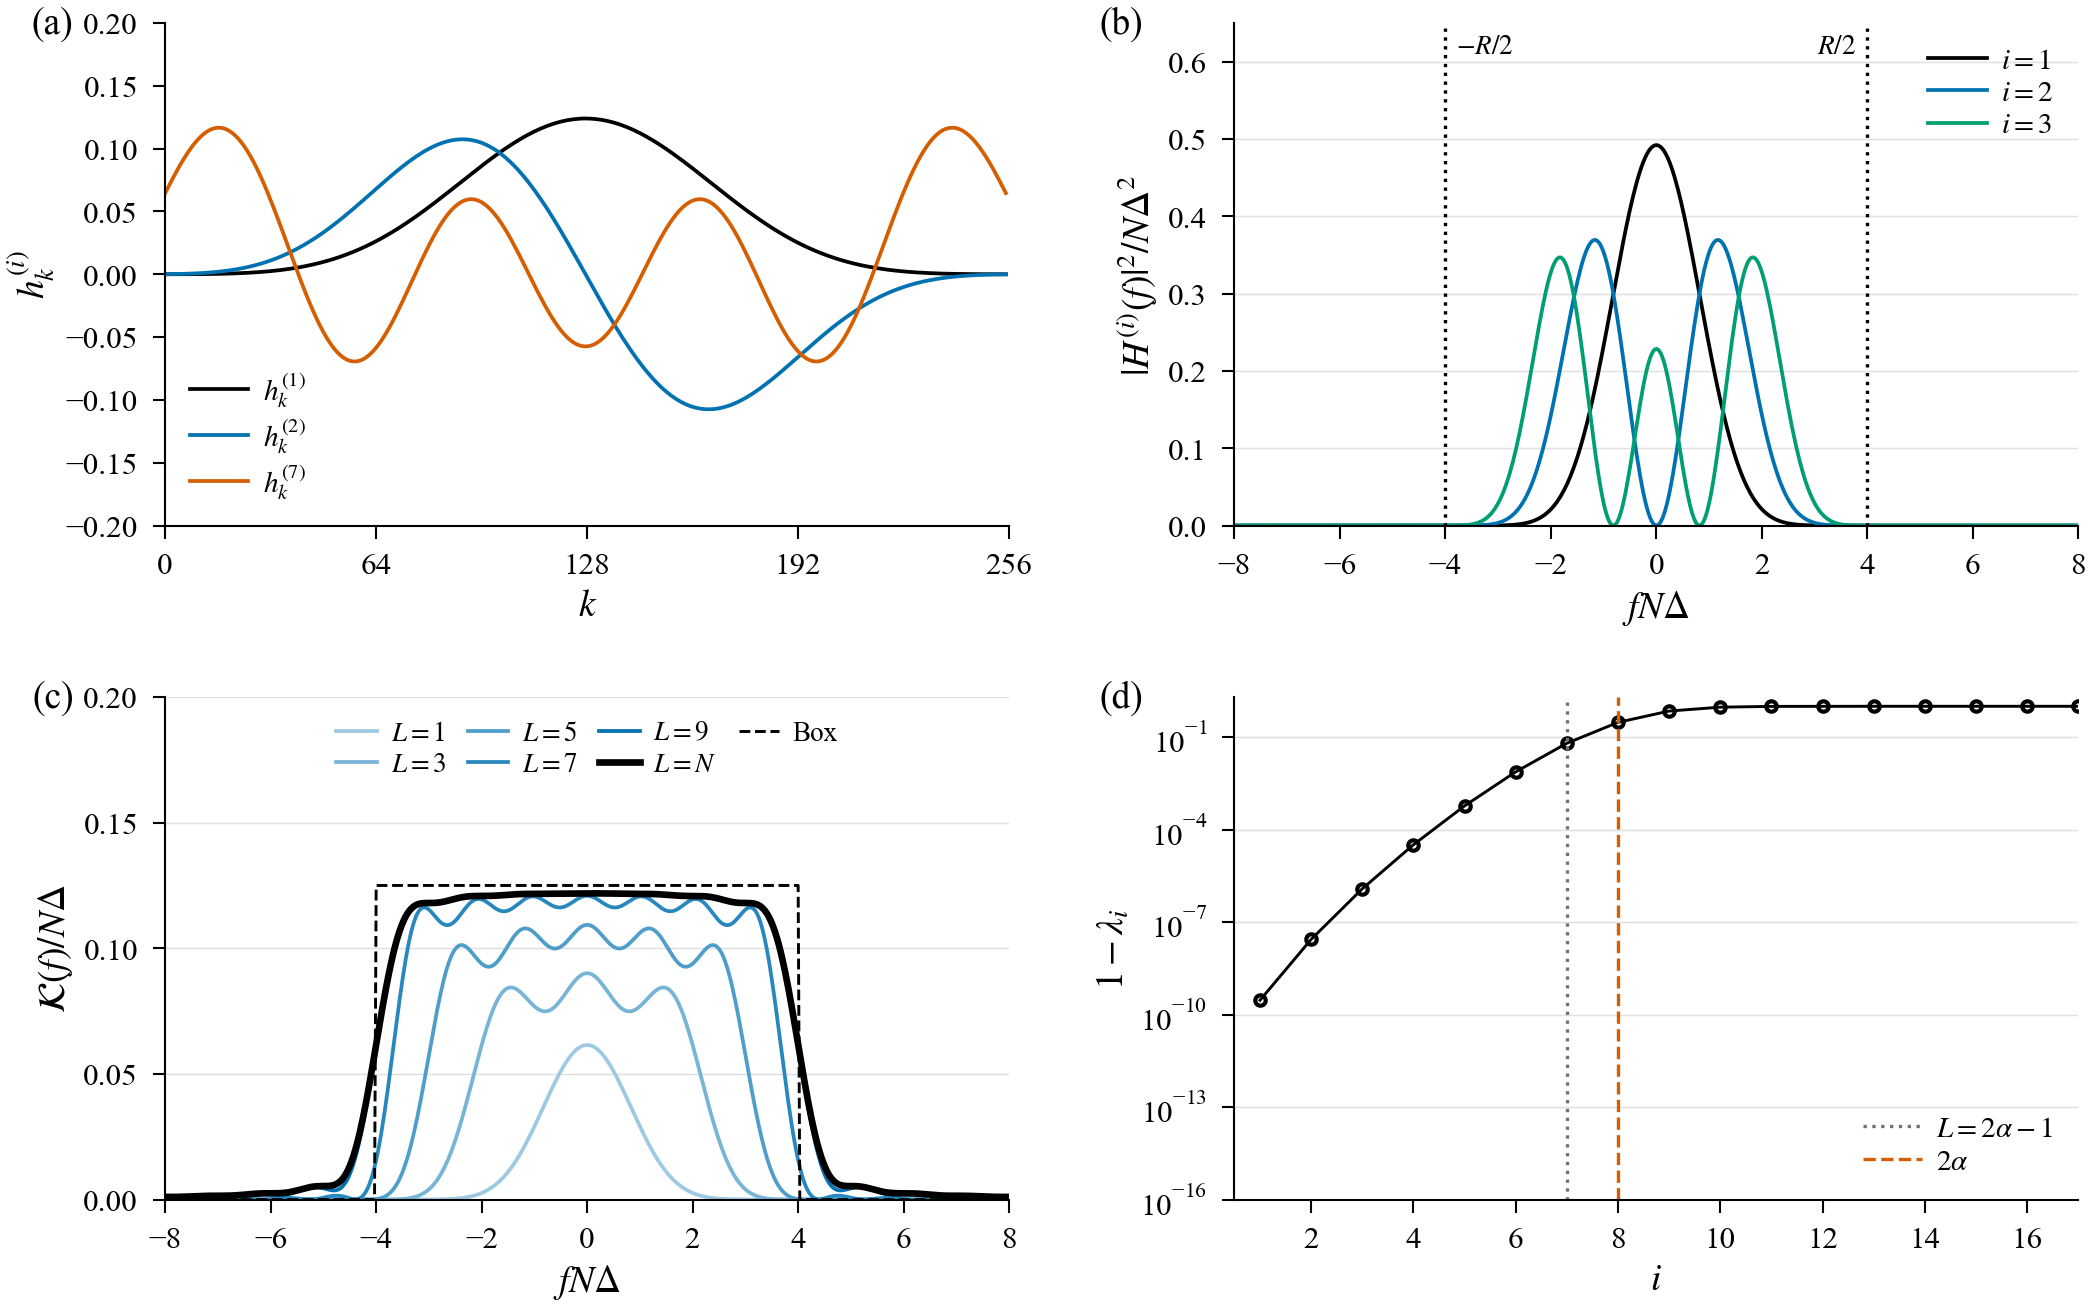
\includegraphics[width=0.92\textwidth]{fig5_slepian_fill.png}
\caption{\textbf{Why the multitaper kernel is a box.} $N=256$, $W=4/N$. (a)~The first six Slepian tapers, offset vertically for display. (b)~Their spectral windows $|U_k(f)|^2$ for unit-norm tapers, each filling the gaps left by the previous ones within the band (shading: $|f|\le W$). (c)~The running sum $\sum_{k<K}\lambda_k|U_k(f)|^2/2NW$ as tapers are added; with all $N$ tapers it is \emph{exactly} the box of half-width $W$ convolved with Fej\'er's kernel, indistinguishable from the box itself (dashed) at this scale, which is the identity \eqref{eq:identity} in kernel form; with the usual $K=2NW-1=7$ it is the box with rounded shoulders and small ripple. (d)~The concentration ladder: the fraction $1-\lambda_k$ of each taper's energy outside the band. Tapers beyond $2NW$ carry only leakage.}
\label{fig:slepian}
\end{figure}

\section{The three methods are one}
\label{sec:one}

\subsection{Every estimator is a bank of tapers}
\label{sec:banks}
Every estimator in this paper is a quadratic form in the data, and every quadratic form is a bank of orthogonal tapers with weights. Write $x_f$ for the data modulated to frequency $f$, with entries $x_te^{-i2\pi ft}$; then $\hat S(f)=x_f^{*}Qx_f$ with a fixed real symmetric matrix $Q$ \cite{percival1993,riedel1995}. A symmetric $Q$ has an eigendecomposition $Q=\sum_kc_kv_kv_k^{\!\top}$ with orthonormal $v_k$, so
\begin{equation}
\hat S(f)=\sum_k c_k\,\bigl|v_k^{\!\top}x_f\bigr|^2 :
\label{eq:bank}
\end{equation}
a bank of orthogonal tapers with weights, which is a multitaper estimate. What distinguishes the methods is how the bank is built (Fig.~\ref{fig:banks}). Averaging periodograms places one window at $M$ offsets and adds the squared transforms with equal weight, $Q=\frac1M\sum_su_su_s^{\!\top}$: a bank of \emph{time-shifted} copies of one window, not orthogonal unless the segments do not overlap. Smoothing a tapered periodogram with a kernel $G$ is $\int G(f')\,|(w\odot e_{f'})^{\!\top}x_f|^2\dd f'$: a bank of \emph{frequency-shifted} copies of one taper, weighted by the kernel. Thomson takes the bank orthogonal from the start.

The bank determines everything. Its kernel is $H=\sum_kc_k|V_k|^2$, and its degrees of freedom at an interior frequency are, to within 3\% for the estimators tested (Appendix~\ref{app:quadratic}; it is Satterthwaite's approximation \cite{satterthwaite1946} applied to the bank),
\begin{equation}
\nu=\frac{2\bigl(\sum_kc_k\bigr)^2}{\sum_kc_k^2},
\label{eq:ladder}
\end{equation}
which equals $2K$ for $K$ equal weights and is smaller whenever the weights are unequal. We call $c_0\ge c_1\ge\dots$ the \emph{eigen-weight ladder}. Thomson's ladder is flat by construction. The ladder of a smoothed single-taper periodogram is sloped, because the modulated copies of one taper overlap heavily in the eigen-basis; this, and nothing specific to Slepian sequences, is why the single-taper route costs variance. The ladder of Welch's method with half-overlapping Hann segments is nearly flat; its cost is in the shape of its kernel.

\begin{figure}[!htb]
\centering
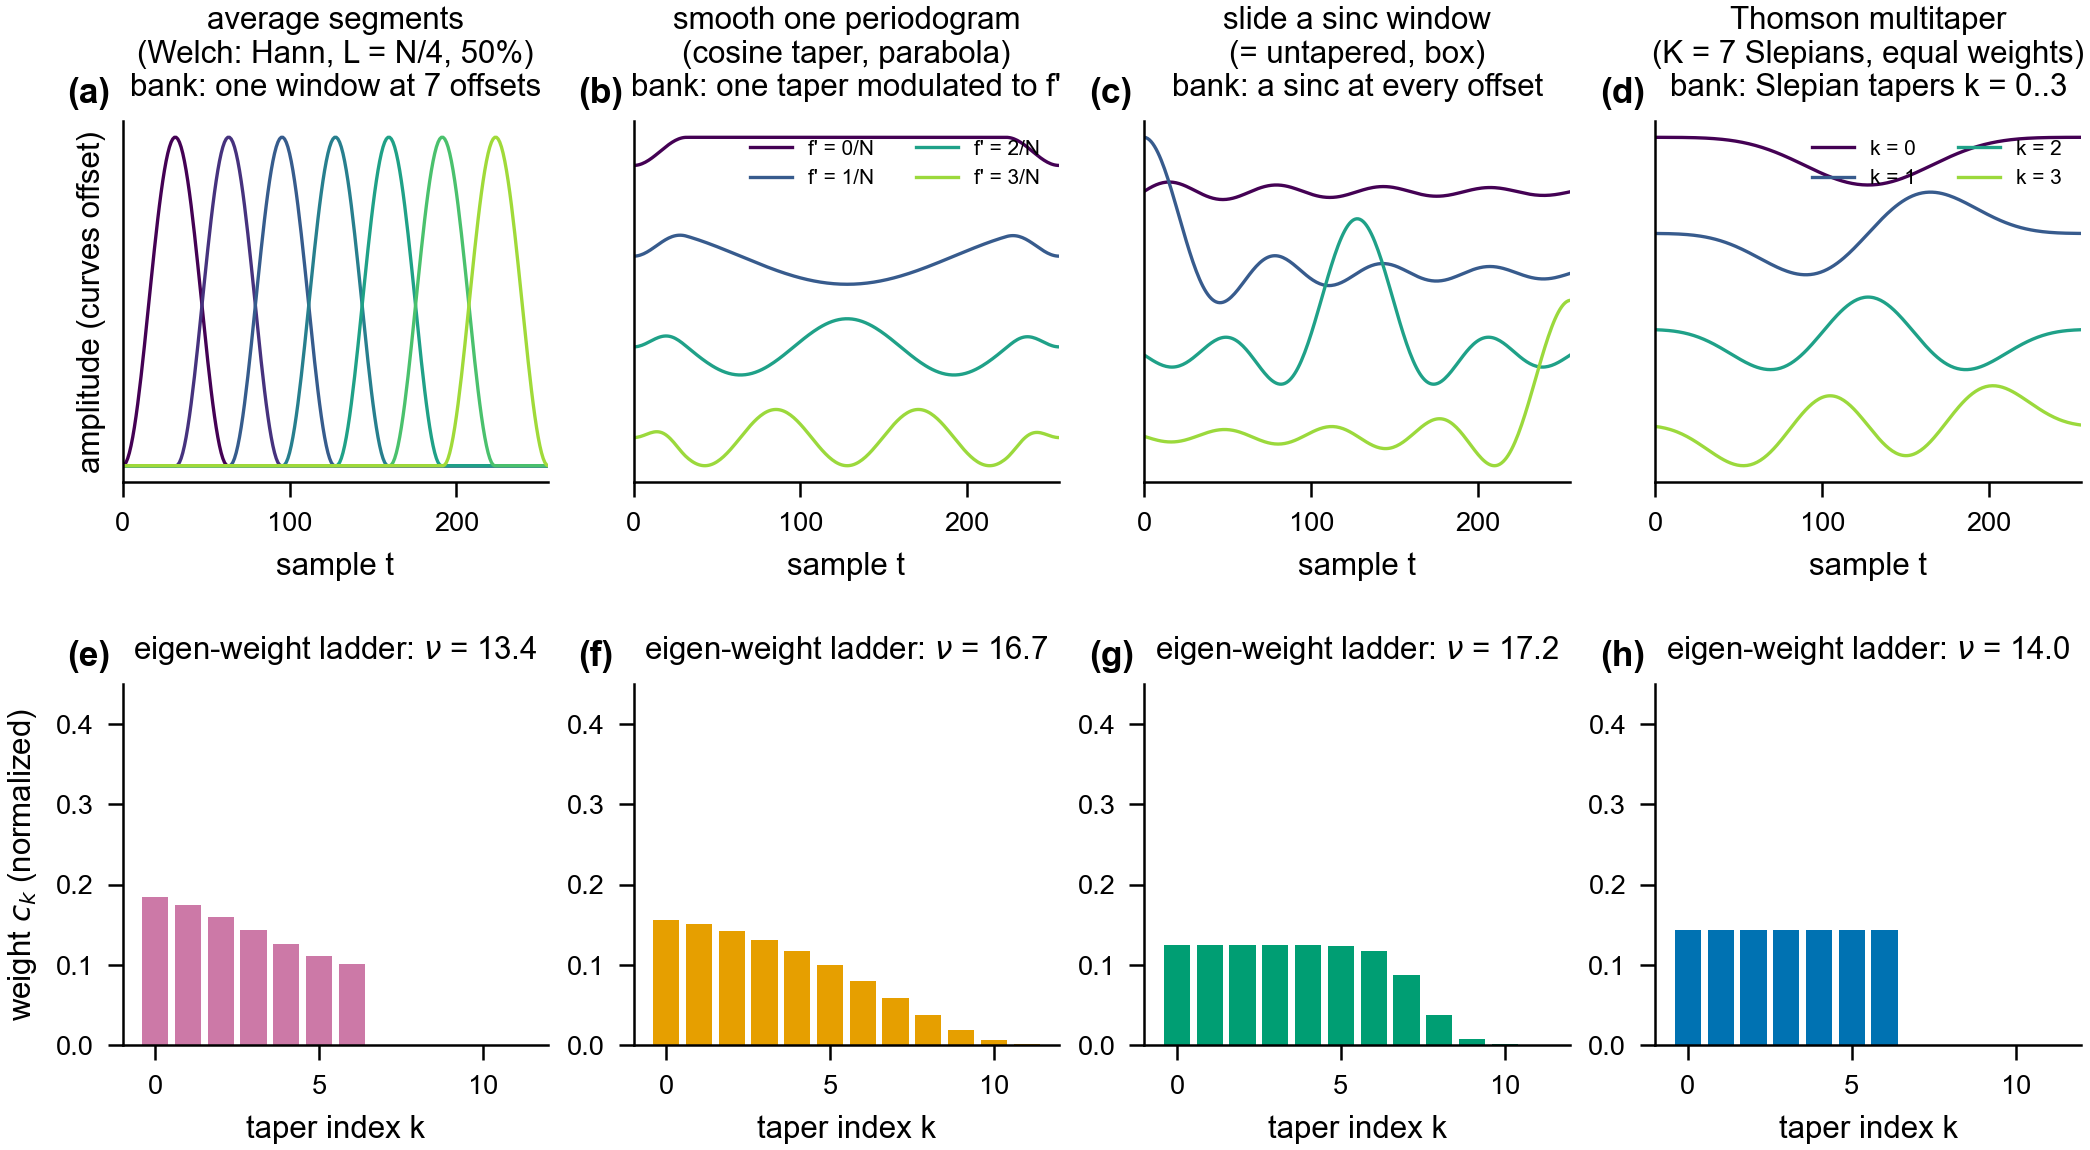
\includegraphics[width=\textwidth]{fig6_taper_banks.png}
\caption{\textbf{Three ways to build a bank of tapers from one window, and the reference bank.} $N=256$, $W=4/N$. (a--d)~The bank as constructed: (a)~Welch's method with Hann segments of length $N/4$ at 50\% overlap (seven time-shifted copies of one window); (b)~a Hann-tapered periodogram smoothed with a Gaussian of standard deviation $3/N$ (frequency-shifted copies of one taper, four of a continuum shown); (c)~a sinc window of half-bandwidth $W$ slid across the record one sample at a time, which in the limit of a long window is exactly the untapered periodogram smoothed with a box and exactly Thomson's estimate with all $N$ tapers weighted by $\lambda_k$; (d)~Thomson's estimate with $K=7$ equally weighted Slepian tapers. (e--h)~The eigen-weight ladder $c_k$ of each, normalized to unit sum, whose flatness sets $\nu=2(\sum_k c_k)^2/\sum_k c_k^2$ by \eqref{eq:ladder}. The eigen-tapers of (c) are the Slepian sequences themselves. Fig.~\ref{fig:banksfull} adds the eigen-tapers and kernels.}
\label{fig:banks}
\end{figure}

\subsection{The identity, and why it is true}
\label{sec:identity}
Keep all $N$ tapers and weight each eigenspectrum by its concentration. Then, exactly,
\begin{equation}
\boxed{\;\frac{1}{2NW}\sum_{k=0}^{N-1}\lambda_k\,\hat S_k(f)\;=\;\frac{1}{2W}\int_{f-W}^{f+W}\hat I(f')\dd f'\;}
\label{eq:identity}
\end{equation}
The left side is the eigenvalue-weighted average of all $N$ eigenspectra (the weights sum to $2NW$). The right side is the periodogram averaged over a box of half-width $W$. This is Thomson's equation (8.3) \cite{thomson1982}; it holds for every record, not just in expectation, and to machine precision (Fig.~\ref{fig:abstract}). The reason is short. The Slepian sequences are the eigenvectors of the $N\times N$ matrix $A$ with entries $\sin(2\pi W(t-t'))/(\pi(t-t'))$, and the $\lambda_k$ are its eigenvalues. That lag sequence, a sinc, is the inverse transform of the box, so $A$ is the box kernel written as a matrix, and $A=\sum_k\lambda_kv_kv_k^{\!\top}$ is that matrix taken apart into orthogonal pieces. Evaluating $x_f^{*}Ax_f$ once through the eigenvectors and once through the lags gives the two sides (Appendix~\ref{app:proof}). In the language of Section~\ref{sec:banks}: \emph{the Slepian tapers are the eigen-tapers of the box-smoothed periodogram}, and their concentrations are its ladder, flat near one for $k<2NW$ and then zero (Fig.~\ref{fig:banks}c).

\subsection{Averaging is smoothing, and the Slepians are principal components}
\label{sec:sliding}
The same matrix arises a third way. Slide a window $w$ across the record one sample at a time, letting it run off both ends of the zero-padded record, and add the squared transforms. Appendix~\ref{app:welch} shows that the resulting $Q$ has entries $r_w(t-t')$, the window's autocorrelation: averaging periodograms of a sliding window is \emph{exactly} the untapered periodogram smoothed with $|\mathcal{W}|^2$. For a sinc window $w_t=2W\,\mathrm{sinc}(2Wt)$ the autocorrelation is $2W\,\mathrm{sinc}(2W\tau)$, the lag sequence of $A$, so
\begin{equation}
\sum_s\bigl|u_s^{\!\top}x_f\bigr|^2=x_f^{*}Ax_f=\sum_k\lambda_k\hat S_k(f),\qquad u_s=\text{the sinc window at offset }s,
\label{eq:sliding}
\end{equation}
exactly for an infinitely long window, with a relative error in $Q$ of 3.5\% for a window of length $2N$, 1.5\% at $4N$ and 0.17\% at $32N$, falling as $1/L$ once $L$ exceeds $2N$ (Appendix~\ref{app:welch}; tested in the repository). Since $A=\sum_su_su_s^{\!\top}$ is the scatter matrix of the shifted windows, its eigenvectors, the Slepian sequences, are the principal components of the sliding sinc window, and Thomson's estimator keeps the leading components.

\subsection{The everyday versions, and what they trade}
\label{sec:everyday}
The standard estimate \eqref{eq:mt} uses equal weights, which is harmless since $\lambda_k\approx1$ for $k<K$, and stops at $K=2NW-1$, which is the whole point. Rearranging \eqref{eq:identity},
\begin{equation}
\frac{K}{2NW}\,\hat S_{\mathrm{mt}}(f)\;\approx\;\underbrace{\frac{1}{2W}\int_{f-W}^{f+W}\hat I(f')\dd f'}_{\text{box-smoothed periodogram}}\;-\;\underbrace{\frac{1}{2NW}\sum_{k\ge K}\lambda_k\hat S_k(f)}_{\text{leaky remainder}} .
\label{eq:corollary}
\end{equation}
The factor $K/2NW$ ($7/8$ for $NW=4$) is only the difference between averaging over $K$ tapers and using weights that sum to $2NW$. The dropped eigenspectra belong to tapers whose energy lies almost entirely outside $[-W,W]$; each contributes at $f$ only what has leaked in from elsewhere. Multitaper estimation is the box-smoothed periodogram, equivalently the sliding-sinc average, with its leakage subtracted. Thomson said as much, noting the two agree ``only for white spectra'' \cite{thomson1982}.

Can either intuitive route perform this subtraction with some other window? Hansson-Sandsten posed the question for Welch's method as a least-squares problem, restructuring the matrix of the Thomson estimator into that of a Welch estimator \cite{hansson2012}. We ran searches of that kind in both families, over segment windows of four lengths and three steps and over taper--kernel pairs by alternating least squares (\texttt{demos/fit\_single\_window.py}). Both return essentially the sliding sinc and the rectangular taper with the box, at a relative distance of $0.27$ to $0.29$ from the $K$-taper matrix against $0.86$ for the Hann taper with the box. Within these families the nearest single-window estimator to Thomson's is the leaky one, and what the intuitive routes can do instead is prevent the leakage by tapering first.

Fig.~\ref{fig:everyday} shows the everyday versions on the record of Fig.~\ref{fig:motif}, Table~\ref{tab:ensemble} scores them over 300 realizations in three regions of the spectrum, Table~\ref{tab:dof} gives their exact kernel properties, and Fig.~\ref{fig:eeg8s} shows them on EEG. Three facts follow: a warning, a price and a surprise.

\begin{figure}[!htb]
\centering
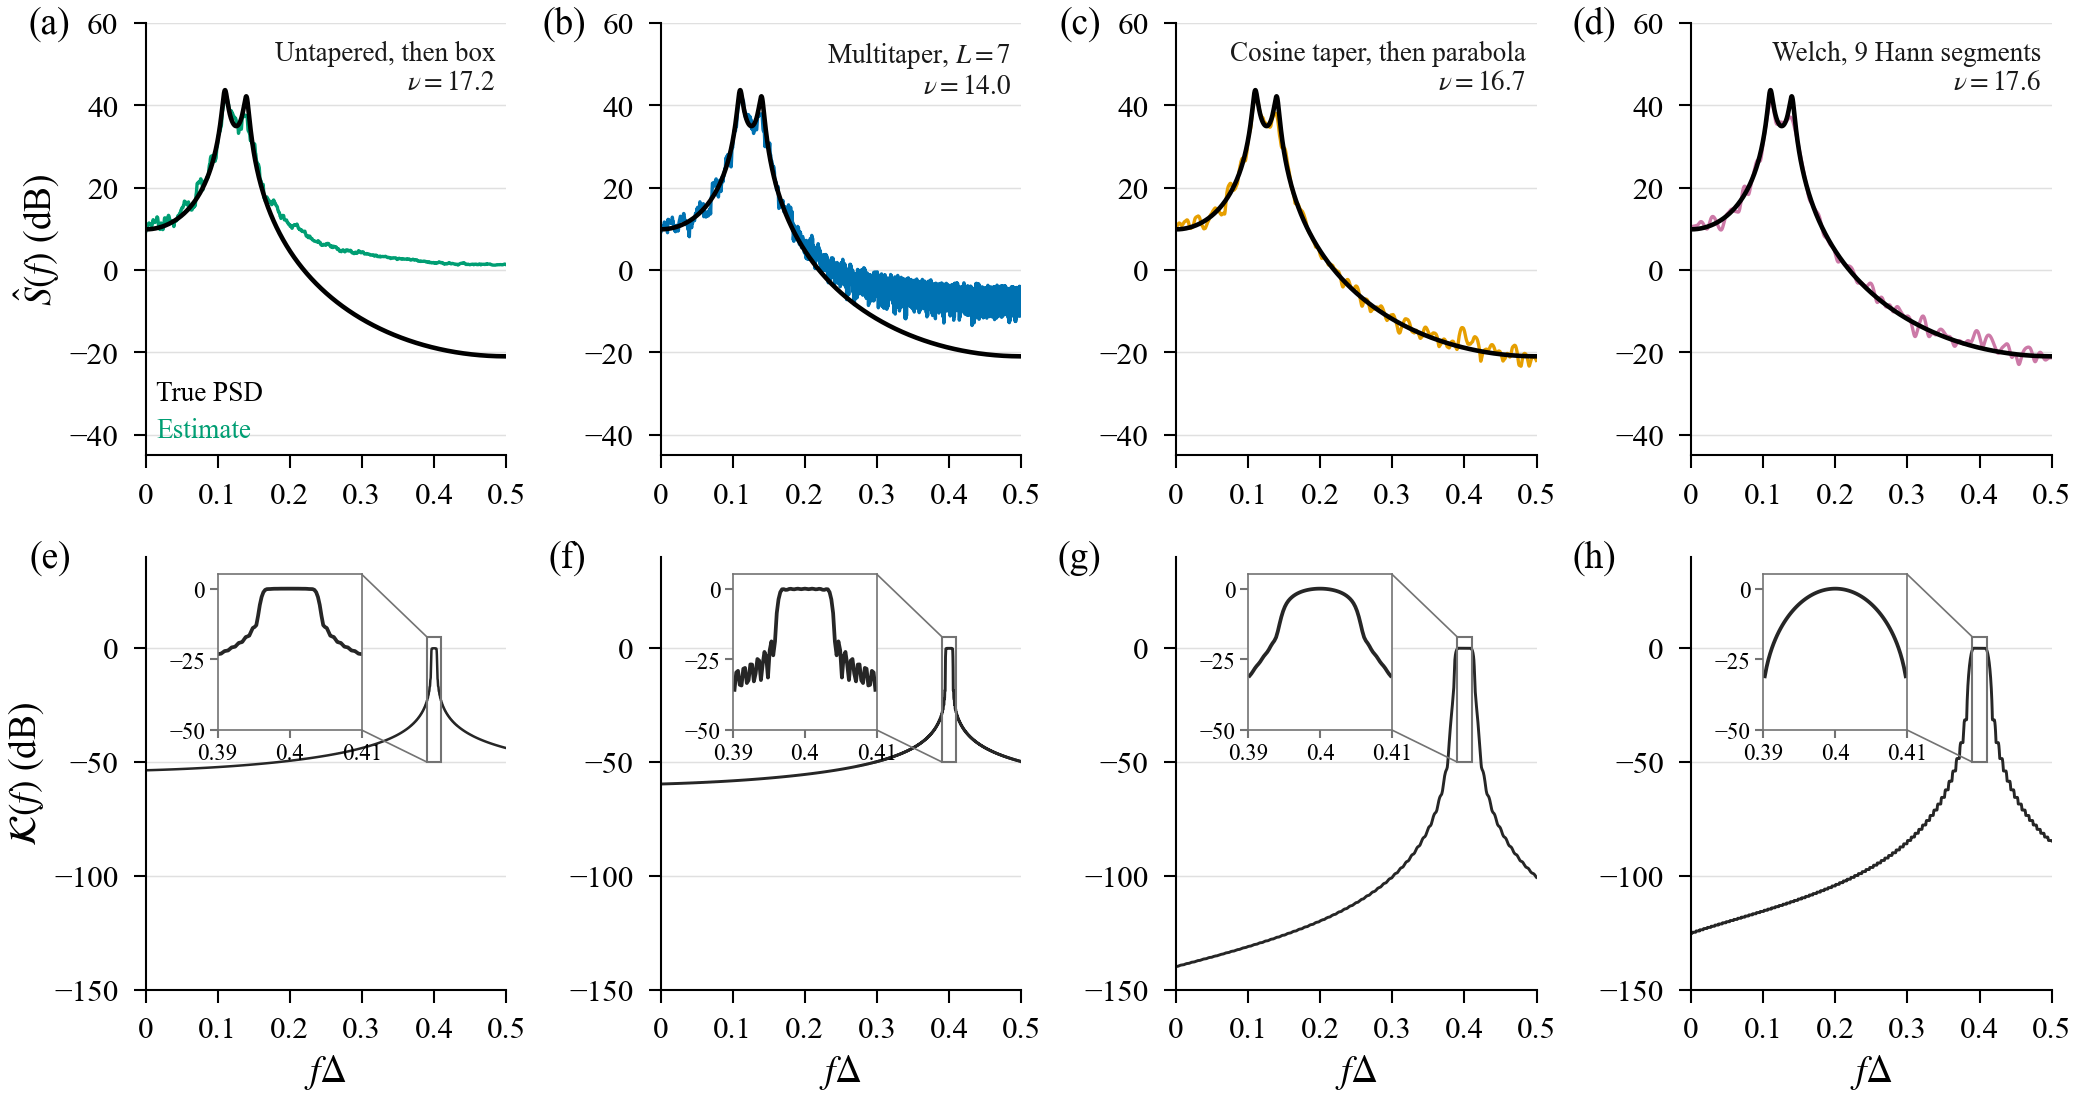
\includegraphics[width=\textwidth]{fig8_everyday_motif.png}
\caption{\textbf{The everyday estimators on the record of Fig.~\ref{fig:motif}} ($N=1024$, $W=4/N$; one realization). (a--d)~The untapered periodogram smoothed with a box, which is the exact estimate \eqref{eq:identity} (green); Thomson's estimate with $K=7$ tapers (blue); a Hann-tapered periodogram smoothed with the same box (orange); and Welch's method with nine Hann segments of 192 samples stepped by 104, chosen for approximately the same half-power width (purple; the four widths are $8.2$, $7.2$, $8.2$ and $7.8/N$). For this realization, an unusually leaky one, the median absolute errors over the band are 11.6, 4.6, 1.3 and 0.8~dB; over 300 realizations they are 5.3, 2.3, 1.4 and 1.0~dB (Table~\ref{tab:ensemble}). (e--h)~The kernels, as in Fig.~\ref{fig:motif}. The untapered box (e) inherits the Fej\'er tails and the estimate floors 20~dB high; the seventh Slepian taper puts the multitaper kernel's skirt at $-22$~dB (f) and the estimate floors 10~dB high; the Hann kernel (g) falls below $-36$~dB beyond the box; Welch's kernel (h) has no flat top and side lobes at the scale of the peaks.}
\label{fig:everyday}
\end{figure}

\begin{table}[!htb]
\centering
\caption{The everyday estimators over 300 realizations of the AR(4) process ($N=1024$, $W=4/N$). Errors are absolute differences in dB between the estimate and the true PSD: the median over the whole band, the root mean square over the peak region ($0.09$ to $0.16$ cycles per sample), and the median where the spectrum is low ($f>0.3$). Widths are half-power widths of the kernel in units of $1/N$. The adaptively weighted estimate has no single kernel; its $\nu$ is $14.0$ at the peaks and $6.5$ for $f>0.3$. Computed by \texttt{demos/everyday\_comparison.py}, which also gives $N=256$ and $N=128$.}
\label{tab:ensemble}
\small
\begin{tabular}{lccccc}
\toprule
Estimator & $\nu$ & width & whole band & peaks & low spectrum\\
\midrule
Untapered periodogram, then box & 17.2 & 8.1 & 5.3 & 1.7 & 13.7\\
Multitaper, $K=7$, equal weights & 14.0 & 7.4 & 2.3 & 1.8 & 6.3\\
Multitaper, $K=6$, equal weights & 12.0 & 6.6 & 1.5 & 2.0 & 2.1\\
Multitaper, $K=7$, adaptive weights & 6.5--14.0 & --- & 1.4 & 1.9 & 1.7\\
Two Slepian tapers ($NW=2$), then box & 13.3 & 8.1 & 1.3 & 1.9 & 1.6\\
Hann periodogram, then box & 8.9 & 8.1 & 1.4 & 2.3 & 1.5\\
Hann periodogram, then box of half-width $6.5/N$ & 14.0 & 13.1 & 1.2 & 2.3 & 1.2\\
Welch, nine Hann segments of 192 samples & 17.6 & 7.6 & 1.0 & 1.8 & 1.0\\
\bottomrule
\end{tabular}
\end{table}

\paragraph{The warning: smoothing and averaging cannot undo leakage.} The box-smoothed untapered periodogram has the right resolution and the most degrees of freedom, and where the spectrum is low it errs by 13.7~dB (Table~\ref{tab:ensemble}), because the leakage in the Fej\'er tails has been averaged, not removed, exactly as \eqref{eq:corollary} predicts. The same box applied to a Hann-tapered periodogram errs by 1.5~dB there. Use a taper for the skirts and a box or a segment length for the top; the latter cannot do the taper's job. Prewhitening, the other classical remedy for a large dynamic range \cite{blackman1958,percival1993}, serves any of the three routes equally.

\paragraph{The price: a single taper costs variance.} At the spectral peaks, where nothing leaks, the errors follow $\nu$: 1.8~dB for the multitaper estimate ($\nu=14.0$) and 2.3~dB for the Hann-tapered, box-smoothed periodogram ($\nu=8.9$, a third fewer, because its ladder is sloped; in relative standard error $\sqrt{2/\nu}$, 47\% against 38\%). The price can instead be paid in resolution: widening the box until the Hann route reaches $\nu=14$ takes a kernel $13/N$ wide where Thomson's is $7.4/N$. The deficit shrinks with $N$, because the extra broadening a single taper imposes scales as $1/N$ while $W$ does not \cite{riedel1994}.

\paragraph{The surprise: the last Slepian taper leaks.} For $NW=4$ the seventh taper has $\lambda_6=0.94$, so 6\% of its energy is outside the band, and it sets the multitaper kernel's skirt at $-22$~dB (Fig.~\ref{fig:everyday}f), well above the Hann taper's $-36$~dB. With the default equal weights and $K=2NW-1$ the multitaper estimate errs by 6.3~dB where the spectrum is low, against 1.5~dB for the Hann route, and on records of 128 samples by 15 against 1.7~dB. Dropping the last taper brings the error to 2.1~dB and Thomson's adaptive weights \cite{thomson1982,thomson1991} to 1.7~dB, by down-weighting the leaky tapers wherever the spectrum is far below its maximum; the cost is that the estimate has $\nu=6.5$ there rather than 14 (Fig.~\ref{fig:ar4}), and recent analysis recommends $K=2NW-O(\log NW)$ for the same reason \cite{karnik2022}. Over the whole band the adaptively weighted estimate and the tapered, smoothed periodogram are then level, at 1.4~dB. The tapered, smoothed periodogram is not a poor cousin of the multitaper estimate: it matches the adaptive estimator where the spectrum is low and gives up a third of the degrees of freedom where it is high.

\paragraph{A remark on Welch's method and on hybrids.} Welch's method with half-overlapping Hann segments matched in half-power width has the most degrees of freedom of any estimator here ($\nu=17.6$, because such segments are nearly orthogonal and its ladder nearly flat) and the smallest errors in Table~\ref{tab:ensemble}. What it pays is kernel shape. The spectral window of a short Hann segment has no flat top and a main lobe whose base, $4/L$, is almost three times its half-power width, so it separates two equal tones only when they are $10.8/N$ apart, against $9.0/N$ for the Hann-tapered box of the same half-power width. Bronez's finding that multitaper estimation beats Welch's method at equal resolution \emph{and} leakage \cite{bronez1992} is the same comparison scored the other way: to give the Welch kernel sharp edges one must lengthen the segments, and then $\nu$ falls below Thomson's. The routes can also be combined. Riedel, Sidorenko and Thomson found a few tapers followed by smoothing best of all on plasma data \cite{riedel1994}, and so it is here: two well-concentrated Slepian tapers ($NW=2$) followed by the box recover $\nu=13.3$ with a side lobe at $-34$~dB and errors of 1.3, 1.9 and 1.6~dB.

\begin{table}[!htb]
\centering
\caption{Exact equivalent degrees of freedom $\nu$ and kernel properties at the same design bandwidth ($N=256$, $W=4/N$, $2NW=8$, $K=7$). Half-power width in units of $1/N$; leakage is the fraction of kernel mass beyond $|f|>2W$ (for the Gaussian, the kernel's own tail); side lobe is the kernel's peak beyond $1.5\times$ the half-power half-width, relative to its maximum. The Welch kernel has no flat top and a main lobe reaching $8/N$. Widths are counted on an FFT grid of 4096 points, which is why the ideal box reads $8.06$ rather than $8$; the figures use finer grids, which moves widths and leakages in the second significant figure. Computed as in Appendix~\ref{app:quadratic}; kernels drawn in Fig.~\ref{fig:kernels}.}
\label{tab:dof}
\begin{tabular}{lcccc}
\toprule
Estimator & $\nu$ & half-power width & leakage & peak side lobe\\
\midrule
Ideal box (reference) & --- & 8.06 & 0 & ---\\
Multitaper, $K=2NW-1=7$, equal weights & 14.0 & 7.44 & 0.0022 & $-22$~dB\\
Multitaper, 7 sine tapers, equal weights & 14.0 & 7.44 & 0.0008 & $-22$~dB\\
Multitaper, all $N$ tapers, weights $\lambda_k$ & 17.2 & 8.06 & 0.0138 & $-17$~dB\\
Untapered periodogram, then box (= sliding sinc) & 17.2 & 8.06 & 0.0138 & $-17$~dB\\
Hann periodogram, then box & 8.9 & 8.06 & $<10^{-4}$ & $-36$~dB\\
Bohman periodogram, then box & 7.3 & 8.06 & $<10^{-4}$ & $-31$~dB\\
Two Slepian tapers ($NW=2$), then box & 13.3 & 8.06 & 0.0002 & $-34$~dB\\
Hann periodogram, then Gaussian ($\sigma=3/N$) & 11.1 & 7.22 & 0.0087 & ---\\
Welch, Hann segments $L=N/4$, 50\% overlap & 13.4 & 5.84 & 0.0005 & $-31$~dB\\
\bottomrule
\end{tabular}
\end{table}

\begin{figure}[!htb]
\centering
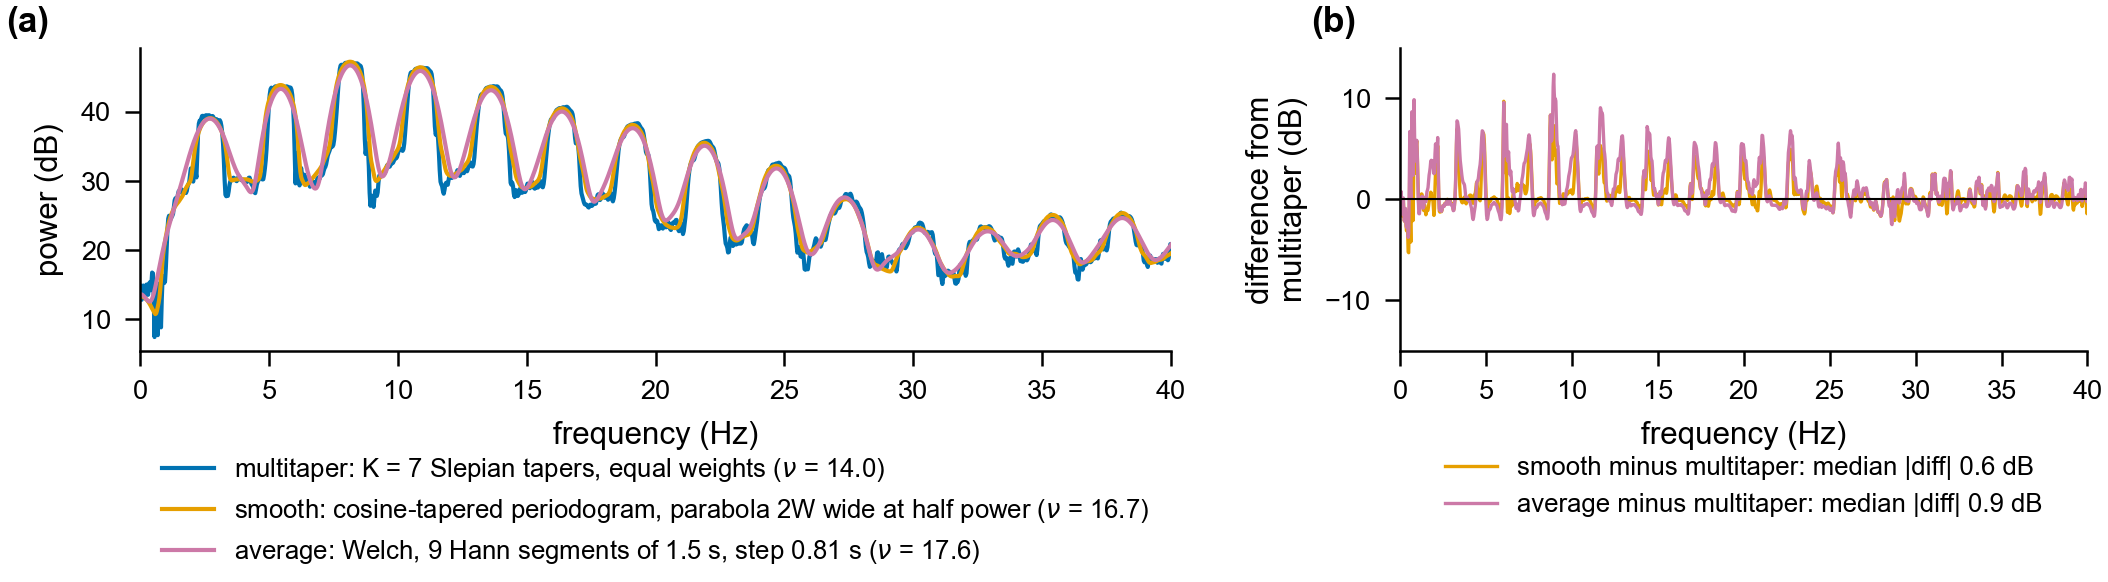
\includegraphics[width=\textwidth]{fig7_everyday_eeg.png}
\caption{\textbf{The everyday versions agree to within their own noise.} (a)~The EEG epoch of Fig.~\ref{fig:abstract} estimated by Thomson's method with $K=7$ tapers ($\nu=14$, blue); by a Hann-tapered periodogram smoothed with the same box ($\nu=8.9$, orange); and by Welch's method with nine Hann segments of $1.5$~s stepped by $0.81$~s ($\nu=17.6$, purple); half-power widths $0.91$, $1.03$ and $0.97$~Hz. (b)~Differences from the multitaper estimate: median absolute difference $1.6$~dB (smoothed) and $0.9$~dB (averaged), 95th percentiles $4.9$ and $5.9$~dB, which is the size of the estimators' own noise ($4.3\sqrt{2/\nu}$ gives $1.6$, $2.1$ and $1.5$~dB). The largest differences are in the valleys between harmonics, which the seventh Slepian taper's side lobes fill in.}
\label{fig:eeg8s}
\end{figure}

\section{A recipe: three routes to one estimate}
\label{sec:recipe}

The three routes are interchangeable, and the choice among them can be made on convenience. Below, $N$ is the number of samples and $2W$ the desired resolution (full width in cycles per sample; divide by the sampling interval for hertz), set to about the width of the narrowest feature that must be preserved (Section~\ref{sec:howwide}).

\begin{framed}
\noindent\textbf{Exact trio.} These give the \emph{same} estimate, to machine precision for (a) and (b) and to a fraction of a decibel for (c); the windows in (b) and (c) are derived from equality with (a) (identity \eqref{eq:identity}, Appendix~\ref{app:welch}).
\begin{enumerate}
\item[(a)] \emph{Multitaper.} All $N$ Slepian tapers for $(N,W)$ with concentrations $\lambda_k$; average the eigenspectra with weights $\lambda_k/2NW$.
\item[(b)] \emph{Smooth.} Periodogram of the untapered record, zero-padded to at least $2N$ points; convolve along frequency with a box of half-width $W$.
\item[(c)] \emph{Average.} A sinc window $w_t=2W\,\mathrm{sinc}(2Wt)$ many times longer than the record, placed at every integer offset including those overhanging the zero-padded ends; sum the squared transforms and divide by $2NW$.
\end{enumerate}
The estimate they share is the leaky one, with the Fej\'er tails of the untapered periodogram.
\end{framed}

\begin{framed}
\noindent\textbf{Everyday trio.} These remove the leakage in three different ways and are therefore close, not identical.
\begin{enumerate}
\item[(a$'$)] \emph{Multitaper.} Keep the $K=2NW-1$ tapers with $\lambda_k\approx1$ and weight them adaptively, or keep $K=2NW-2$ with equal weights. Expect $\nu\approx2K$ where the spectrum is high and about half that where it is far below its maximum.
\item[(b$'$)] \emph{Smooth.} Multiply by a Hann window scaled to unit energy (a Bohman window has a higher first side lobe, $-31$ against $-36$~dB, but far skirts that fall faster, Fig.~\ref{fig:tradeoff}b, at a further cost in $\nu$); squared FFT, zero-padded to at least $2N$ (more only for a finer display grid); convolve with a box of half-width $W$ (or a Gaussian of standard deviation about $0.8W$, which has a comparable half-power width). Expect a half-power width of about $2W$ once $2W$ exceeds a few $/N$, a first side lobe at $-36$~dB, and $\nu\approx0.55$ to $0.6$ times $2\cdot2NW$. Two Slepian tapers at half the time--bandwidth product in place of the Hann window nearly double $\nu$.
\item[(c$'$)] \emph{Average.} Hann-tapered segments of length $L\approx1.4/(2W)$, overlapping by half; average their periodograms. Expect $\nu$ about twice the number of segments, a kernel with no flat top whose main lobe has base $4/L$, almost three times its half-power width, and leakage set by the Hann window of length $L$.
\end{enumerate}
\end{framed}

Prefer (a$'$) when the record is so short that every degree of freedom counts ($2NW\lesssim6$), when Thomson's F-test for lines is wanted, or for coherence and cross-spectra, where an orthogonal bank has advantages a single taper does not share \cite{walden2000}. Prefer (b$'$) when interpretability matters, when the bandwidth should vary with frequency (wider at high frequencies is sensible and awkward to express in tapers or segments), and for time--frequency displays where smoothing across both axes is natural. Prefer (c$'$) when the record is long and a pipeline already computes it; it has the most degrees of freedom at matched half-power width and the poorest two-tone resolution. Whichever route is used, its $\nu$ gives the error bar: the 95\% confidence interval of Section~\ref{sec:periodogram} runs from $-3.3$ to $+5.3$~dB around the estimate for $\nu=8.9$ and from $-2.7$ to $+4.0$~dB for $\nu=14$.

\section{EEG demonstration: seizures}
\label{sec:eeg}

\paragraph{Data and settings.} Figs.~\ref{fig:eeg} and \ref{fig:eeg2} apply the everyday trio to two ten-minute scalp EEG clips containing focal seizures, the setting in which spectrograms are read clinically. The clips are de-identified recordings from a seizure-annotation set (ELROND) drawn from the Brain Data Science Platform, sampled at 200~Hz on 20 channels, with seizure onsets and offsets as marked by one of the authors (M.B.W.); one channel of each is shown, the one with the largest ictal rise in 2 to 20~Hz power. The features that must survive are the harmonics of the ictal rhythm. Measured on the Hann periodogram at the ictal instant of Fig.~\ref{fig:eeg}, the fundamental is at $7.7$~Hz, the harmonics are $7.4$~Hz apart, and each peak is $0.9$~Hz wide in a 2-second window, which is the resolution of the window rather than of the rhythm; in the second clip the spacing falls to about 4~Hz as the seizure slows. By the rule of Section~\ref{sec:howwide} the bandwidth should be well under the harmonic spacing and otherwise as wide as possible, and we set $2W=2$~Hz in 2-second windows: multitaper with $NW=2$, $K=3$ and equal weights; a Hann taper with a box of half-width 1~Hz; Welch's method with 0.7-second segments.

\paragraph{Results.} In Fig.~\ref{fig:eeg} the ictal rhythm begins near 7.5~Hz with harmonics to 25~Hz and slows over a minute, the ``chirp'' that marks an evolving seizure, and ends in post-ictal suppression; Fig.~\ref{fig:eeg2} has two such seizures, each a harmonic stack descending from 20~Hz to 3~Hz. (These descriptions are readings of the spectrograms.) The unsmoothed periodogram shows the chirps through heavy noise; the multitaper and smoothed-periodogram spectrograms are indistinguishable by eye, and the spectra at a pre-ictal and an ictal instant (Fig.~\ref{fig:eeg}d,\,f) show all three everyday estimators resolving the same harmonics. Over all $599$ windows the two spectrograms differ by a median of $1.5$~dB (Fig.~\ref{fig:eeg}h) and $1.2$~dB (Fig.~\ref{fig:eeg2}), within the estimators' own noise at $\nu=6$ and $\nu\approx5$ ($2.5$ and $2.8$~dB), since the two estimates share most of it. Band powers, the quantity most analyses report, agree more closely still, because integrating over a band averages the noise that distinguishes the estimators (Table~\ref{tab:bandpower}): the ictal rise in theta, alpha and beta power in Fig.~\ref{fig:eeg} is 17 to 18~dB by every estimator, within $0.7$~dB of one another, and the per-window disagreement with the multitaper estimate is about $1$~dB for the Hann route and $0.5$~dB for Welch's method. Whatever a study concludes from band powers, it would conclude by any of the three routes.

\begin{figure}[!htb]
\centering
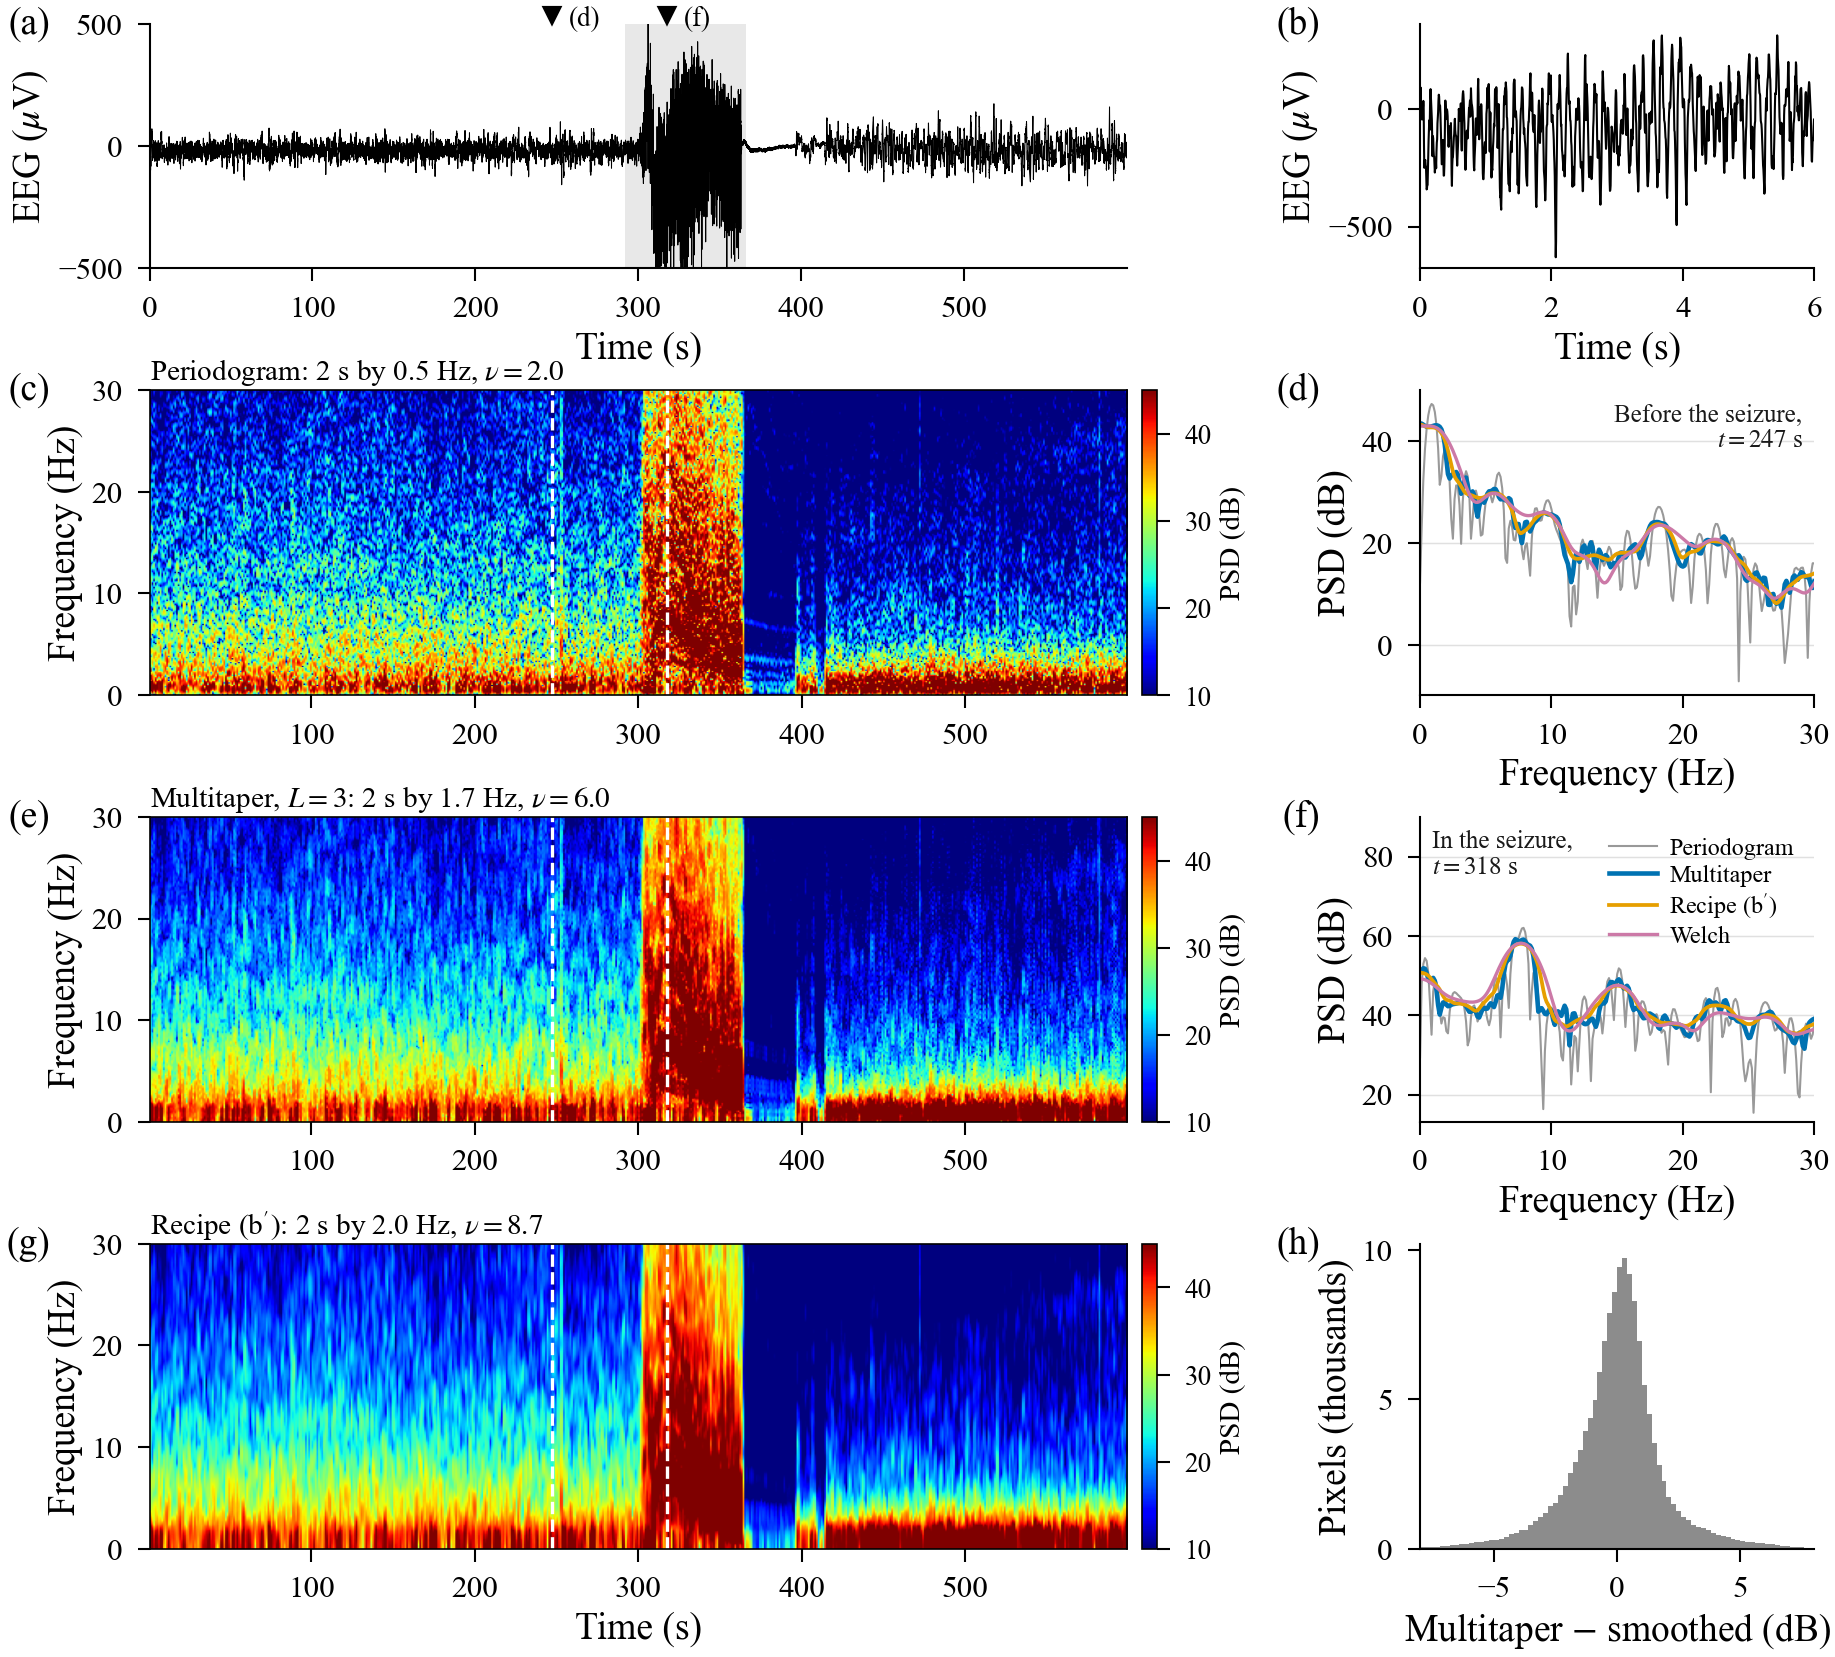
\includegraphics[width=\textwidth]{fig10_eeg_seizure.png}
\caption{\textbf{Three estimators of a seizure.} (a)~Ten minutes of de-identified scalp EEG at 200~Hz (ELROND seizure-annotation set), channel C4 against the common average, displayed between $\pm500~\mu$V; the seizure is shaded and the dashed lines mark the instants used in (d) and (f). (b)~Six seconds of the ictal rhythm from $t=318$~s. (c,\,e,\,g)~Spectrograms from 599 windows of 2~s stepped by 1~s: the Hann periodogram ($\nu=2$), the multitaper estimate with $NW=2$, $K=3$ ($\nu=6$), and the Hann periodogram smoothed with a box of half-width $W=1$~Hz ($\nu=4.8$), on one colour scale of 10 to 45~dB shared with Fig.~\ref{fig:eeg2}. (d,\,f)~Spectra at the pre-ictal and ictal instants by all three, plus Welch's method with 0.7-second Hann segments ($\nu=7.7$). (h)~Distribution over all pixels of the difference between (e) and (g). The channel is the one with the largest ictal rise in 2 to 20~Hz power.}
\label{fig:eeg}
\end{figure}

\begin{figure}[!htb]
\centering
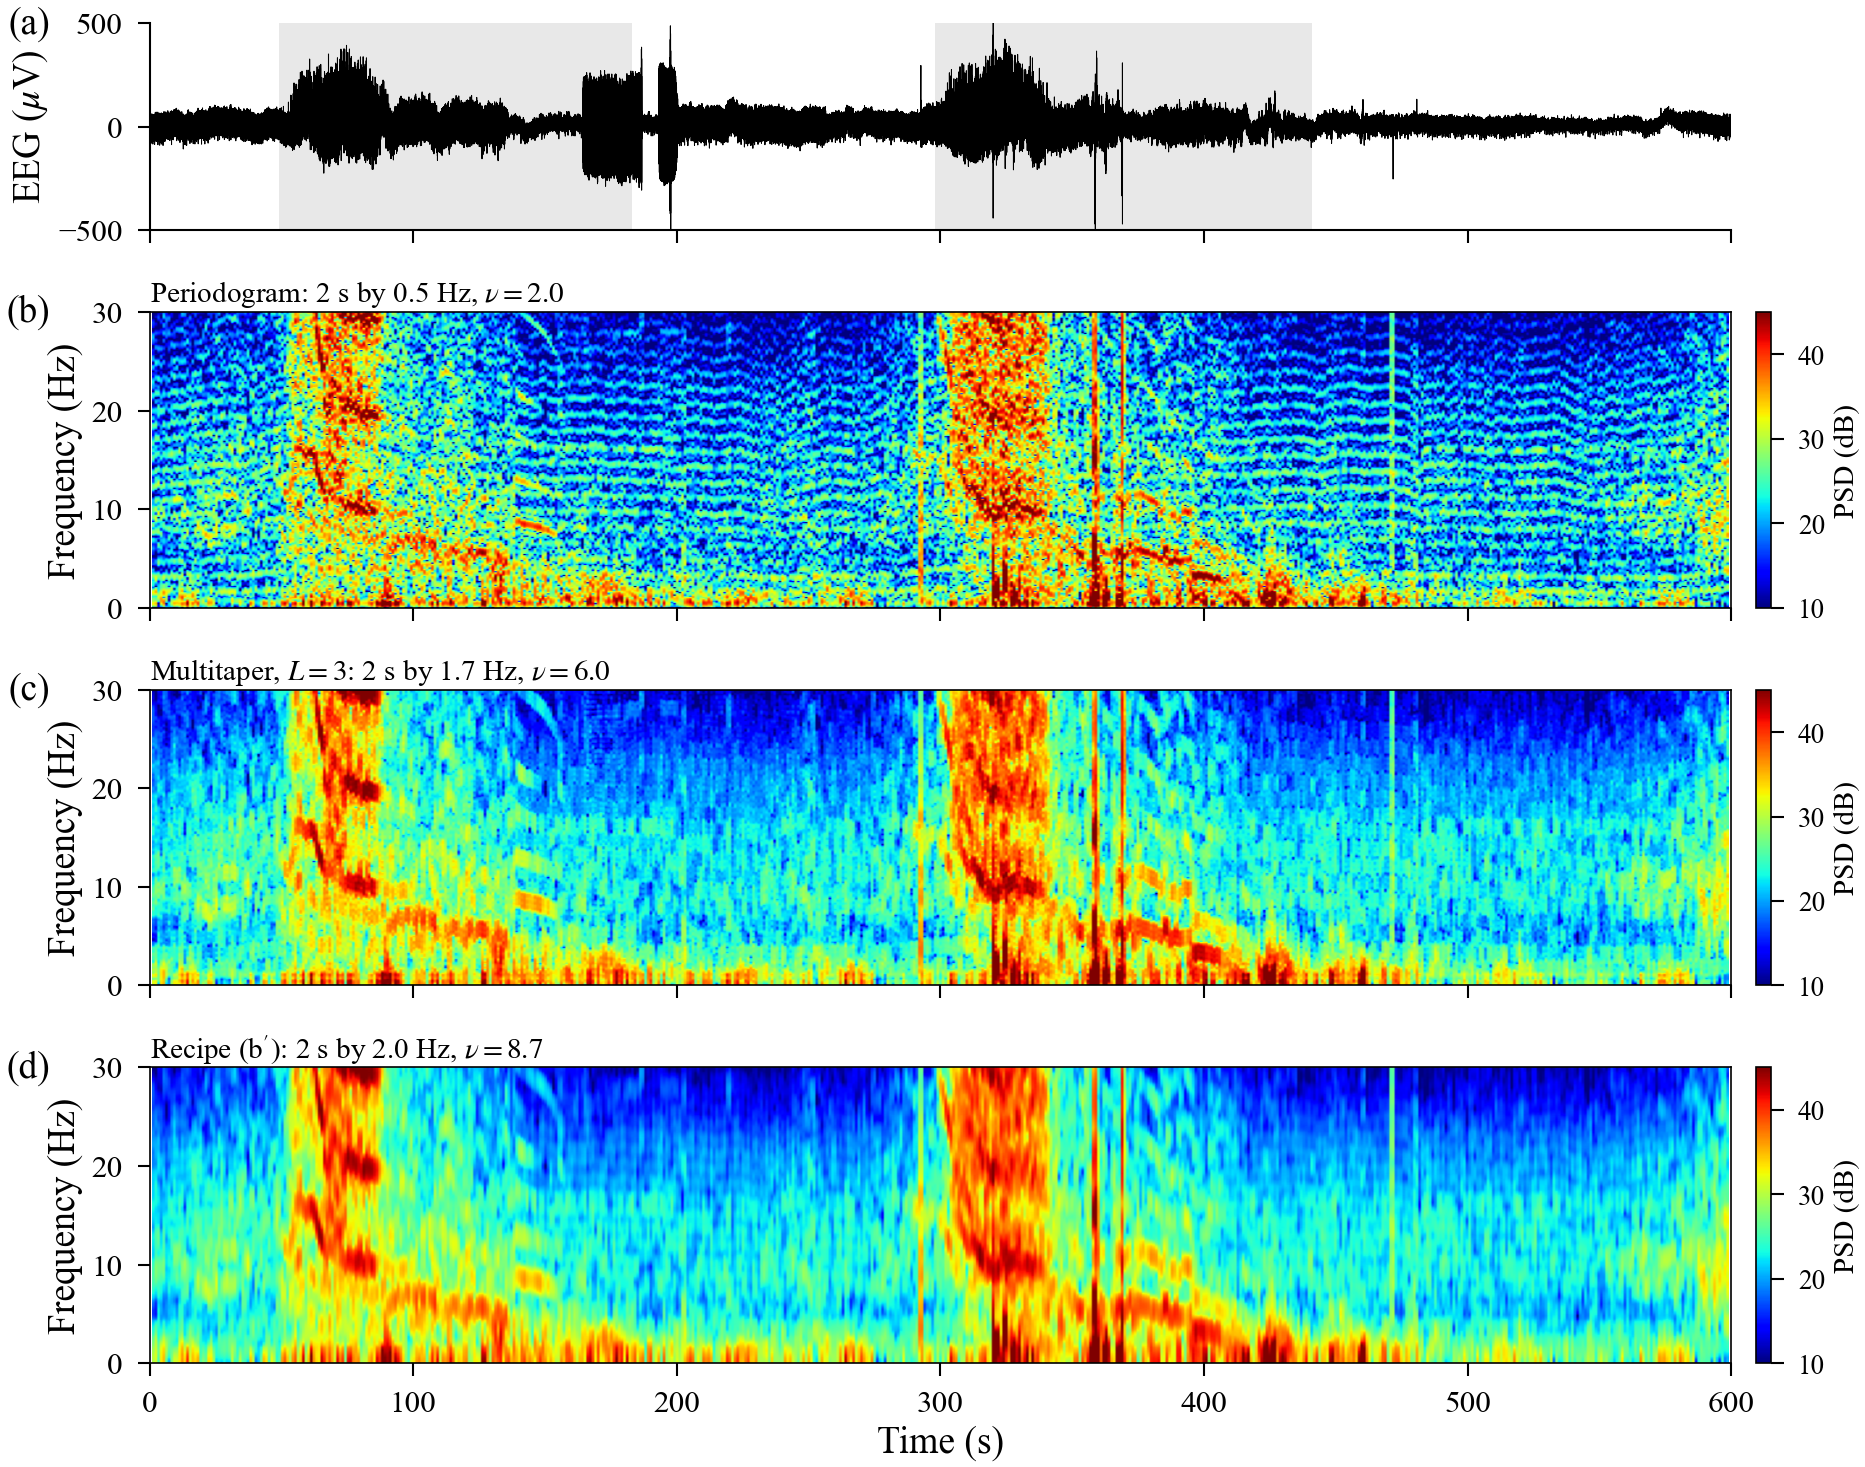
\includegraphics[width=\textwidth]{fig11_eeg_two_seizures.png}
\caption{\textbf{Two seizures in one clip.} (a)~Ten minutes of de-identified scalp EEG (ELROND set), channel Fp1 against the common average, displayed between $\pm500~\mu$V, both seizures shaded. (b--d)~Spectrograms as in Fig.~\ref{fig:eeg}, 599 windows of 2~s stepped by 1~s, same colour scale: the Hann periodogram ($\nu=2$), the multitaper estimate with $NW=2$, $K=3$ ($\nu=6$), and the Hann periodogram smoothed with a box of half-width 1~Hz ($\nu=4.8$). Each seizure is a harmonic stack that descends from about 20~Hz to 3~Hz over two minutes; the two smoothed estimators render it identically and the unsmoothed periodogram renders it through noise.}
\label{fig:eeg2}
\end{figure}

\begin{table}[!htb]
\centering
\caption{Band powers from the everyday estimators on the two seizure clips, one channel each, 599 windows of 2~s per clip (75 ictal and 120 pre-ictal windows for Fig.~\ref{fig:eeg}; 279 and 43 for Fig.~\ref{fig:eeg2}). Left: the mean ictal band power minus the mean pre-ictal band power (the windows in the two minutes before the first seizure, of which the second clip has only 43), in dB, by each estimator. Right: the median over all windows of the absolute difference between each estimator's band power and the multitaper estimate's, in dB. Bandwidth $2W=2$~Hz throughout ($NW=2$; box half-width 1~Hz; 0.7-second Welch segments).}
\label{tab:bandpower}
\small
\begin{tabular}{llccccc|cccc}
\toprule
clip & band & periodogram & multitaper & Hann+box & recipe (b$'$) & Welch & periodogram & Hann+box & recipe (b$'$) & Welch\\
 & & \multicolumn{5}{c|}{ictal minus pre-ictal band power (dB)} & \multicolumn{4}{c}{median $|$difference from multitaper$|$ per window (dB)}\\
\midrule
Fig.~\ref{fig:eeg} (C4) & delta (1--4 Hz) & +6.3 & +6.3 & +6.3 & +6.4 & +6.3 & 1.39 & 1.08 & 0.23 & 0.61\\
 & theta (4--8 Hz) & +17.9 & +17.8 & +17.7 & +17.6 & +17.6 & 1.15 & 0.97 & 0.31 & 0.64\\
 & alpha (8--13 Hz) & +17.4 & +18.0 & +17.6 & +18.1 & +18.1 & 1.06 & 0.97 & 0.26 & 0.61\\
 & beta (13--30 Hz) & +17.5 & +17.7 & +17.5 & +17.8 & +17.8 & 0.71 & 0.67 & 0.16 & 0.38\\
\midrule
Fig.~\ref{fig:eeg2} (Fp1) & delta (1--4 Hz) & +7.3 & +8.1 & +7.8 & +8.3 & +8.2 & 1.25 & 0.95 & 0.28 & 0.73\\
 & theta (4--8 Hz) & +7.8 & +7.7 & +7.8 & +7.8 & +7.7 & 0.89 & 0.78 & 0.19 & 0.56\\
 & alpha (8--13 Hz) & +4.1 & +4.4 & +4.2 & +4.5 & +4.5 & 0.66 & 0.58 & 0.12 & 0.44\\
 & beta (13--30 Hz) & +5.5 & +5.6 & +5.4 & +5.5 & +5.5 & 0.42 & 0.41 & 0.11 & 0.38\\
\bottomrule
\end{tabular}


\end{table}

\section{Relation to prior work}
\label{sec:prior}

\paragraph{What is known.} The pieces of this account are old; what has been missing is their assembly in a place that users read. Identity \eqref{eq:identity} is Thomson's equation (8.3) \cite{thomson1982}, half a page in a forty-page paper. That any quadratic estimator is a weighted multitaper estimator whose tapers are the eigenvectors of its matrix is textbook material \cite{percival1993}, developed for kernel smoothers by Riedel and Sidorenko \cite{riedel1995} and for multivariate estimators by Walden \cite{walden2000}, and the degrees-of-freedom formula \eqref{eq:ladder} is Satterthwaite's approximation \cite{satterthwaite1946} applied to that decomposition. That averaging periodograms of a sliding window smooths the periodogram is Welch's \cite{welch1967}, in the general time-and-lag-weighting form of Nuttall and Carter \cite{nuttall1982}, and Hansson-Sandsten restructured the Thomson estimator's matrix into a Welch estimator by least squares for real-time use \cite{hansson2012}. Abreu and Romero proved the convergence of the $K$-taper kernel to a box with a rate \cite{abreu2017}, and Karnik, Romberg and Davenport use \eqref{eq:identity} in matrix form for a fast multitaper algorithm \cite{karnik2022}. Empirical comparisons are those of Riedel, Sidorenko and Thomson against smoothed tapered periodograms \cite{riedel1994} and of Bronez against Welch's method \cite{bronez1992}; window properties are catalogued by Harris \cite{harris1978}. These results live in the vocabulary of eigenvalue problems, error rates and matrix algorithms, while the texts from which neuroscientists learn spectral estimation \cite{mitra1999,bokil2010,babadi2014,prerau2017,kay1988} present the methods side by side rather than as one.

\paragraph{What we add.} We assemble these results into one picture, the bank of tapers, and draw its consequences for practice. The sliding-window form of the identity, with the Slepian sequences as principal components of a sliding sinc window, gives the averaging route its exact place. The eigen-weight ladder turns a standard degrees-of-freedom formula into an explanation: the variance cost of a single taper is the slope of its ladder. Tables~\ref{tab:dof} and \ref{tab:ensemble} say what each route costs and where each wins, the adaptively weighted estimate included. The bandwidth rule and the recipes make the choice of parameters a matter of looking at the data. The paper belongs to the genre of Bruns's demonstration that Fourier, Hilbert and wavelet analyses of neural signals are one method \cite{bruns2004}, and the same picture places those methods too: a Morlet scalogram is a single-taper periodogram whose Gaussian taper shortens as frequency rises.

\section{Limitations}
\emph{Scope of the identity.} The identity is exact for the eigenvalue-weighted estimate with all $N$ tapers, and its sliding-window form only in the limit of a long window; the everyday trio are close, not equal, and the paper quantifies the difference rather than removing it. \emph{Scope of the comparison.} Table~\ref{tab:ensemble} is one process, a fourth-order autoregression with two peaks and a 65~dB range, compared at matched design bandwidth rather than matched $\nu$; its whole-band median is dominated by the low-power region, where leakage lives, which is why the table also scores the peaks, where the ranking reverses. Other spectra, line components and very short records will rank the routes differently, and the adaptive weights are Thomson's original iteration, without the jackknife or quadratic-inverse refinements \cite{thomson1991}. \emph{Assumptions.} Kernels, degrees of freedom and leakage are properties of the estimators for a stationary Gaussian process, computed on a finite FFT grid; the spectrograms assume stationarity within each 2-second window, which a seizure violates at its onset. \emph{Evidence.} The EEG evidence is two clips and one channel of each, with equal-weight multitaper estimates. \emph{Not treated.} Coherence and cross-spectra, inference beyond the $\chi^2_\nu$ interval, and data-driven bandwidth selection.

\section{Conclusion}
Averaging periodograms, smoothing a periodogram and multitaper estimation are one estimator, a bank of tapers with weights, built three ways from one window. The multitaper estimate is exactly a smoothed periodogram when all Slepian tapers are used with their eigenvalues as weights, and, in the limit of a long window, exactly an average of sliding-window periodograms; the everyday version is the same thing with its leaky components removed. Seen this way, its parameters become ones users already understand (a taper for the skirts, a box or a segment length for the width), the bandwidth becomes a balance of blur against noise, and the hand-rolled routes are seen for what they are: with a taper, as good on leakage as an adaptively weighted multitaper estimate and a third short on degrees of freedom; without one, wrong. For most EEG work any of the three is fine, and knowing they are the same is what lets one choose on grounds of convenience.

\section*{Data and code availability}
All figures are generated by the scripts in the accompanying repository (\texttt{specsmooth} Python package; \texttt{demos/make\_figures.py}, \texttt{demos/everyday\_comparison.py}, \texttt{demos/band\_power\_table.py}, \texttt{demos/fit\_single\_window.py}), where the identities \eqref{eq:identity} and \eqref{eq:sliding}, the sliding-window convergence at $L=N$ to $32N$, the formulas of Appendix~\ref{app:quadratic} and their Monte Carlo checks are implemented as tests. The simulated data and the 128~Hz EEG epoch of Figs.~\ref{fig:abstract} and \ref{fig:eeg8s} are included; the two seizure clips are de-identified clinical recordings from the Brain Data Science Platform and are available to credentialed users under its data-use agreement, and the scripts print every number quoted from them; their printed output is committed under \texttt{demos/outputs/}.

\appendix

\section{Proof of the identity \eqref{eq:identity}}
\label{app:proof}
Let $A$ be the $N\times N$ matrix with entries $A_{tt'}=\sin(2\pi W(t-t'))/(\pi(t-t'))$ and $A_{tt}=2W$. The Slepian sequences are its eigenvectors, $Av_k=\lambda_kv_k$, $\|v_k\|=1$ \cite{slepian1978}, so $A=\sum_k\lambda_kv_kv_k^{\!\top}$ and $\sum_k\lambda_k=\operatorname{tr}A=2NW$. With $x_f$ the modulated data, $\hat S_k(f)=|v_k^{\!\top}x_f|^2$, and
\begin{align}
\sum_{k}\lambda_k\hat S_k(f)
&=x_f^{*}\Bigl(\sum_k\lambda_kv_kv_k^{\!\top}\Bigr)x_f
=\sum_{t,t'}A_{tt'}\,x_tx_{t'}\,e^{-i2\pi f(t-t')}
=\sum_{\tau=-(N-1)}^{N-1}h_\tau\,\hat s_\tau\,e^{-i2\pi f\tau},
\end{align}
with $h_\tau=\sin(2\pi W\tau)/(\pi\tau)$ and $\hat s_\tau=\sum_tx_tx_{t+\tau}$, collecting terms by lag. Now $\hat s_\tau$ is the inverse transform of $N\hat I(f)$ and $h_\tau$ the inverse transform of the indicator of $[-W,W]$; a product of lag sequences transforms to a convolution in frequency, so the sum equals $\int_{f-W}^{f+W}N\hat I(f')\dd f'$. Divide by $2NW$. $\square$

\section{Kernels, banks and variance of quadratic estimators}
\label{app:quadratic}
Every estimator in this paper is $\hat S(f)=x_f^{*}Qx_f$ with $Q$ real symmetric positive semidefinite and independent of $f$ \cite{percival1993,riedel1995}: $Q=\sum_kc_kv_kv_k^{\!\top}$ for a multitaper estimate; $Q_{tt'}=w_tg_{t-t'}w_{t'}$ for a periodogram tapered with $w$ and smoothed with the lag window $g$ (the inverse transform of the kernel); $Q=\sum_su_su_s^{\!\top}/\sum_s\|u_s\|^2$ for averaged periodograms of a window placed at offsets $s$.

\emph{Bank.} $Q=\sum_kc_kv_kv_k^{\!\top}$ with orthonormal $v_k$ and $c_k\ge0$, so every $Q$ is a multitaper estimate \eqref{eq:bank}.

\emph{Kernel.} $\E[\hat S(f)]=\int H(f-f')S(f')\dd f'$ with $H$ the transform of the lag sums $q_\tau=\sum_tQ_{t,t+\tau}$; equivalently $H=\sum_kc_k|V_k|^2$. For a tapered, smoothed periodogram $H=|\mathcal{W}|^2*G$; for averaged periodograms $H=|\mathcal{W}_L|^2$ whatever the overlap; for $Q=A$, $H=B_W*F$, which is why two rows of Table~\ref{tab:dof} coincide.

\emph{Degrees of freedom.} For unit white Gaussian noise, $\hat S(f)$ has mean $\operatorname{tr}Q_f$ and variance $2\operatorname{tr}Q_f^2$, with $Q_f$ the real part of $Q$ conjugated by the modulation, so $\nu=(\operatorname{tr}Q_f)^2/\operatorname{tr}Q_f^2$, the chi-square approximation of Satterthwaite \cite{satterthwaite1946}. At an interior frequency each modulated taper is orthogonal to its conjugate, each term of the bank is an independent $\chi^2_2$, and $\nu=2(\sum c_k)^2/\sum c_k^2$, equation~\eqref{eq:ladder}. The two formulas agree to within 3\% for the three estimators tested (multitaper, Hann-then-box and Welch); Table~\ref{tab:dof} uses the first, and Monte Carlo on white noise (3000 draws) agrees with it to within 15\% for the same three (repository tests).

\emph{Resolution and leakage.} Resolution is the half-power full width of $H$; leakage is the fraction of $H$ outside a stated band; the peak side lobe is the maximum of $H$ beyond $1.5\times$ the half-power half-width. A practitioner's convolution of a zero-padded periodogram with a kernel on the same grid is exactly the lag-window estimate above once the padding reaches $2N$ points, because the periodogram's lag sequence vanishes beyond $|\tau|=N-1$.

\section{Averaging over a sliding window is smoothing}
\label{app:welch}

\subsection*{C.1 Continuous time: the limit of all overlaps}
Let $x(t)$ be the record, zero outside $[0,T]$, with transform $X(\omega)$, and $w$ a real symmetric window with transform $W$. Windowing at shift $\tau$ gives $s_\tau(t)=x(t)w(t-\tau)$, with transform $S_\tau(\omega)=\frac{1}{2\pi}\int X(\omega')W(\omega-\omega')e^{-i(\omega-\omega')\tau}\dd\omega'$. Welch's method with shifts $n\Delta$ averages $|S_{n\Delta}(\omega)|^2$ over $n$. Let the overlap grow without bound, $\Delta\to0$: the average becomes a Riemann sum for an integral over the shift, which can be evaluated in closed form,
\begin{align}
\int_{-\infty}^{\infty}|S_\tau(\omega)|^2\dd\tau
&=\frac{1}{(2\pi)^2}\iint X(\omega')X^{*}(\omega'')W(\omega-\omega')W^{*}(\omega-\omega'')\Bigl[\int_{-\infty}^{\infty}e^{\,i(\omega'-\omega'')\tau}\dd\tau\Bigr]\dd\omega'\dd\omega''\notag\\
&=\frac{1}{2\pi}\int|X(\omega')|^2\,|W(\omega-\omega')|^2\dd\omega'=\frac{1}{2\pi}\bigl(|W|^2*|X|^2\bigr)(\omega),
\label{eq:continuous}
\end{align}
because the bracket is $2\pi\delta(\omega'-\omega'')$. The sum of the periodograms of all shifted windows is the raw periodogram smoothed with the window's own spectral window; dividing by $T\!\int\!w^2$, the trace of the quadratic form, makes the estimate unbiased for white noise. Two remarks. The shift integral must run over every $\tau$ at which the window touches the record, including shifts at which it overhangs the ends; that is what produces the delta function, and restricting $\tau$ to $[0,T]$ leaves an edge term that vanishes only when $T$ is much longer than the window. And for a Gaussian window of standard deviation $\sigma_t$ the kernel is Gaussian with standard deviation $1/(2\sqrt2\,\pi\sigma_t)$ cycles per unit time: sliding a Gaussian window is smoothing with a Gaussian. This calculation, with a Gaussian window, was the content of an unpublished 2001 note by one of us, written before the connection to multitaper estimation was known; the result is Welch's \cite{welch1967} and is contained in Nuttall and Carter's framework \cite{nuttall1982}.

\subsection*{C.2 Discrete time, finite record: exact, with no limit}
In discrete time the shift is an integer and the sum over all shifts is exact rather than a limit. Let $w$ have length $L$ and $u_s$ be the length-$N$ vector holding $w$ at offset $s$, with the parts of $w$ outside the record discarded. Averaging over offsets gives $Q_{tt'}=\sum_sw[t-s]w[t'-s]$. If the offsets run over every integer for which the window touches the record, $s=-(L-1),\dots,N-1$, the sum equals the autocorrelation $r_w(t-t')$ for every pair inside the record, so $Q$ is Toeplitz and the estimator is the lag-window estimate of the untapered periodogram with lag window $r_w$ and kernel $|\mathcal{W}(f)|^2$. This is exact for a finite record; with a larger step or without overhang it holds approximately in the interior. The equivalence is for the \emph{untapered} periodogram: a tapered periodogram that is then smoothed has $Q_{tt'}=w_tg_{t-t'}w_{t'}$, which is not Toeplitz and is not the average of any single sliding window, though it is a time-and-lag weighting in the sense of \cite{nuttall1982}. For the sinc window, $r_w(\tau)\to2W\,\mathrm{sinc}(2W\tau)$ as $L\to\infty$, the lag sequence of $A$; the relative error in $Q$ falls as $1/L$ because the truncated sinc's autocorrelation differs from the sinc by a term of that order. Hence \eqref{eq:sliding}, and the Slepian sequences are the principal components of the shifted sinc windows.

\section{Supplementary figures}
\label{app:supp}
\renewcommand{\thefigure}{S\arabic{figure}}
\setcounter{figure}{0}

\begin{figure}[!htb]
\centering
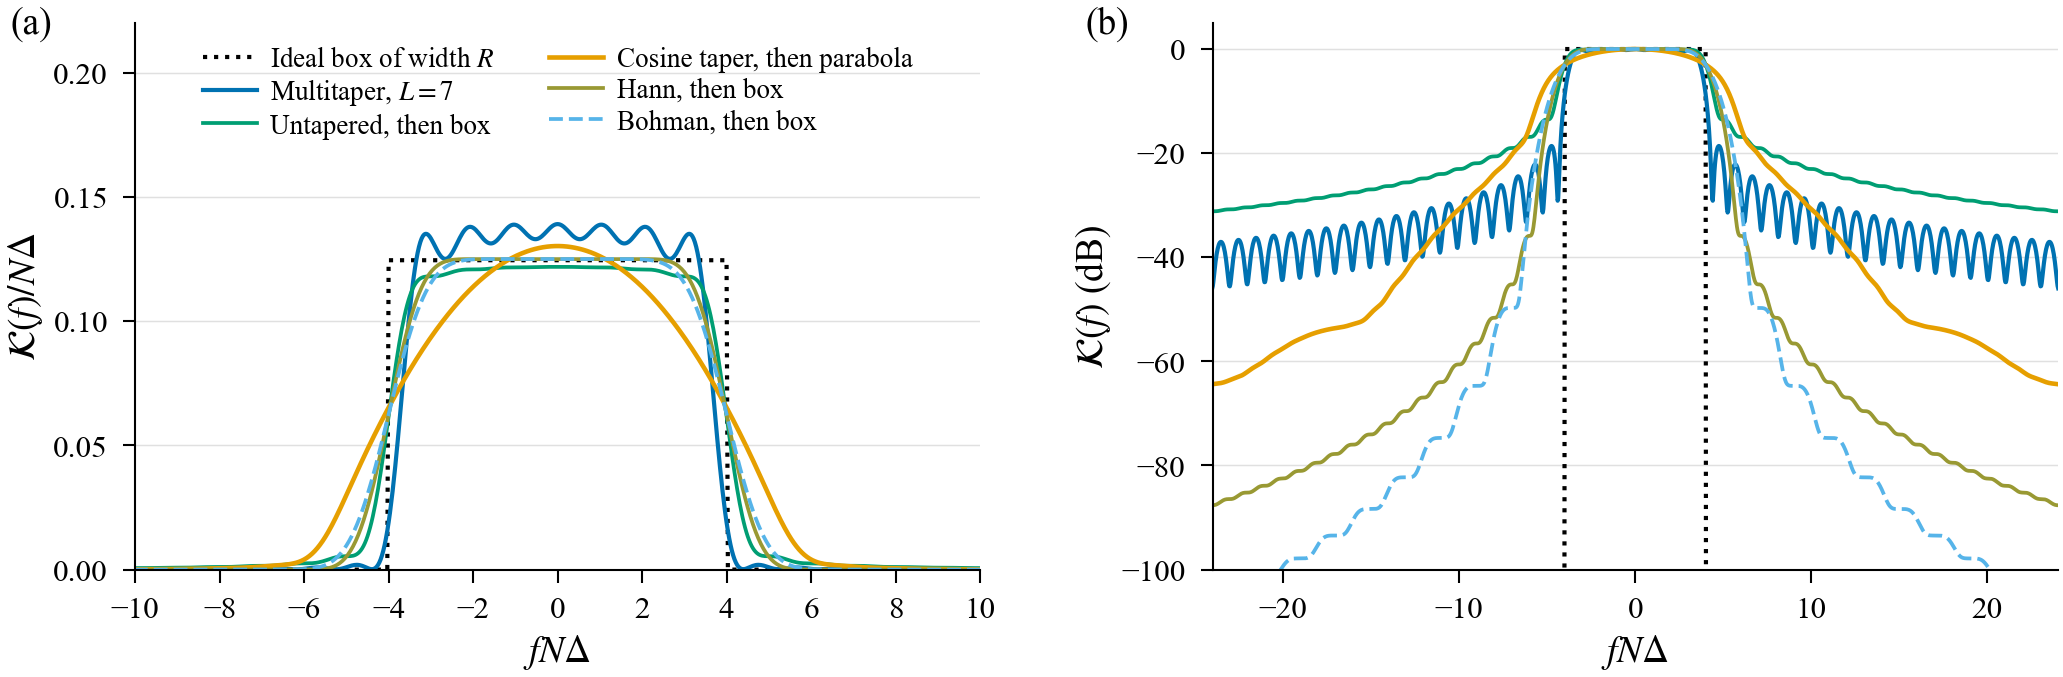
\includegraphics[width=\textwidth]{fig1_kernels.png}
\caption{\textbf{Kernels at the same design bandwidth} ($N=256$, $W=4/N$; Table~\ref{tab:dof}): (a)~on a linear scale near the main lobe and (b)~in dB relative to the peak. The ideal box; the $K=7$ multitaper kernel ($\nu=14.0$); and the untapered ($\nu=17.2$), Hann ($\nu=8.9$) and Bohman ($\nu=7.3$) periodograms followed by the box. All main lobes have nearly the same width; the skirts differ by 40~dB.}
\label{fig:kernels}
\end{figure}

\begin{figure}[!htb]
\centering
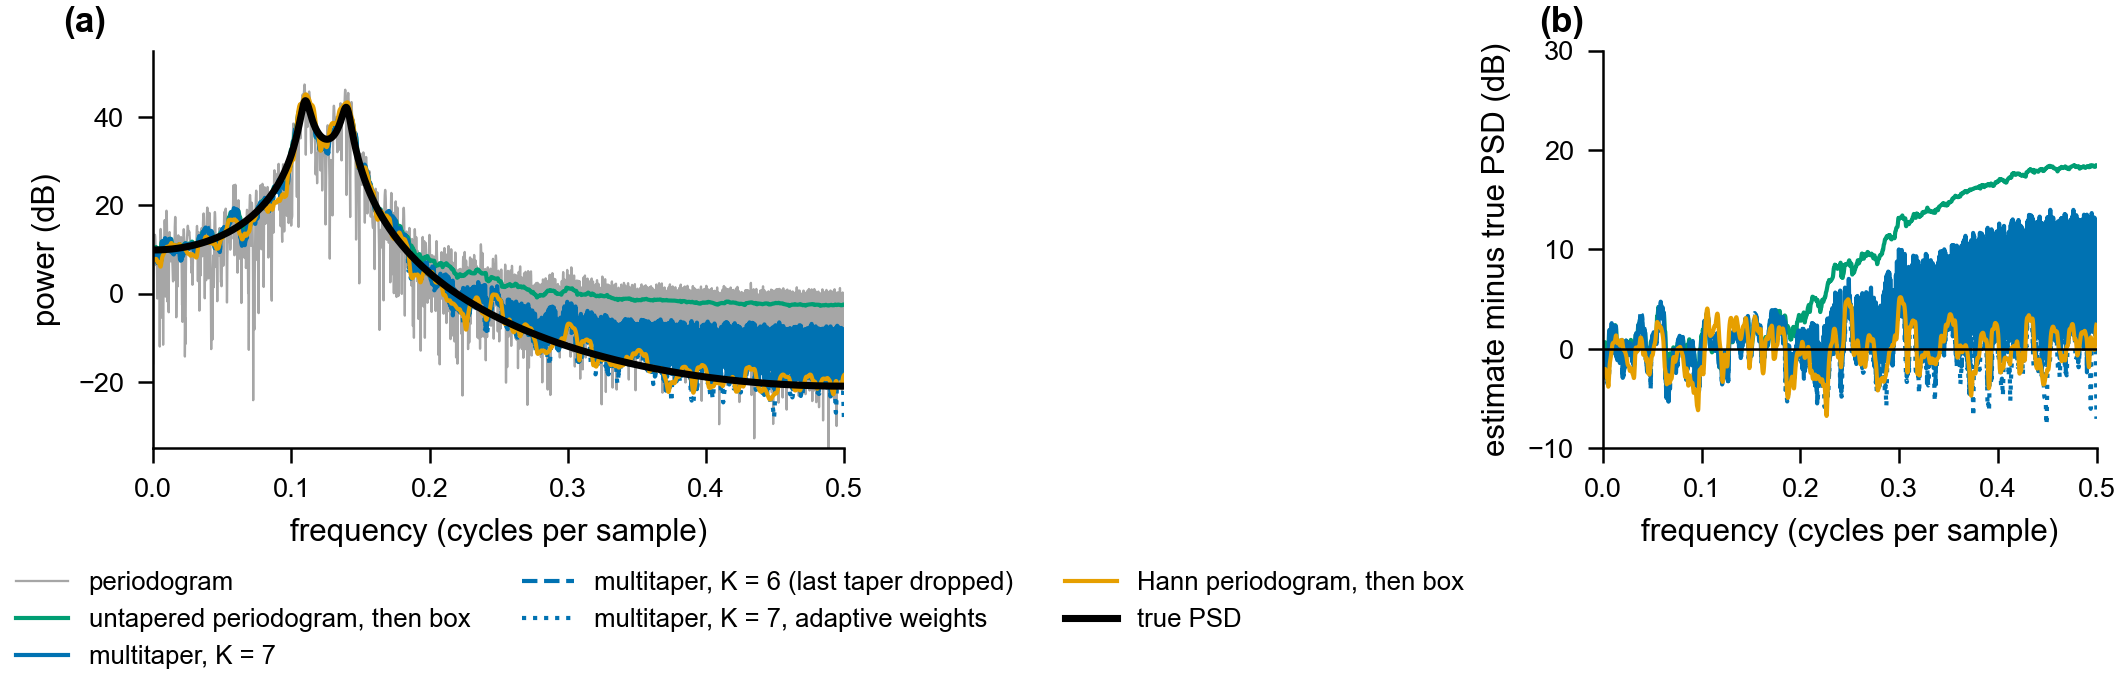
\includegraphics[width=0.8\textwidth]{fig2_ar4_leakage.png}
\caption{\textbf{Dropping the leakiest taper.} (a)~One realization of the AR(4) process ($N=1024$, $W=4/N$): the periodogram ($\nu=2$, grey); the untapered periodogram smoothed with the box ($\nu=17.2$, green); the equal-weight multitaper estimate with $K=7$ ($\nu=14$, solid blue) and with $K=6$ ($\nu=12$, dashed blue), and the adaptively weighted estimate with $K=7$ (dotted blue); the Hann-tapered periodogram smoothed with the box ($\nu=8.9$, orange); and the true PSD (black). (b)~Each smoothed estimate minus the true PSD: the untapered box floors 20~dB high, $K=7$ floors 10~dB high, dropping the seventh taper halves that, and the adaptive weights and the Hann route track the truth.}
\label{fig:ar4}
\end{figure}

\begin{figure}[!htb]
\centering
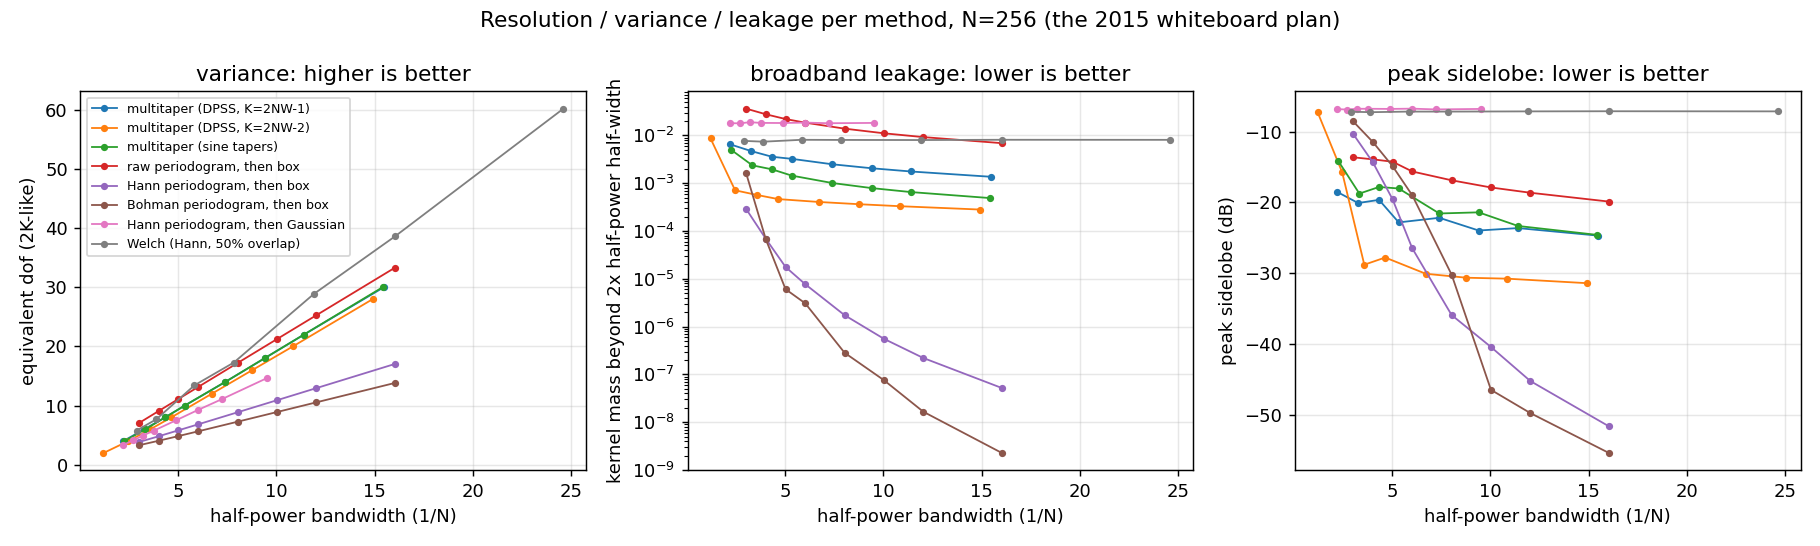
\includegraphics[width=\textwidth]{fig3_tradeoff.png}
\caption{\textbf{Variance, leakage and side-lobe level versus measured resolution} for $N=256$; all curves are exact kernel and degrees-of-freedom computations (no sampling variability). Each method's bandwidth parameter is swept and the quantities are plotted against the resulting half-power width, so methods are compared at equal resolution: multitaper with $K=2NW-1$ and $2NW-2$ Slepian tapers and with sine tapers; untapered, Hann and Bohman periodograms followed by a box; a Hann periodogram followed by a Gaussian; Welch's method with 50\% overlap. (a)~Equivalent degrees of freedom $\nu$ (higher means less variance). (b)~Kernel power beyond twice the half-power half-width. (c)~The kernel's peak beyond $1.5\times$ the half-power half-width; for the Gaussian and Welch kernels, which have no flat top, this reports the main-lobe skirt rather than a side lobe. The dotted line marks the $8/N$ width of Table~\ref{tab:dof}.}
\label{fig:tradeoff}
\end{figure}

\begin{figure}[!htb]
\centering
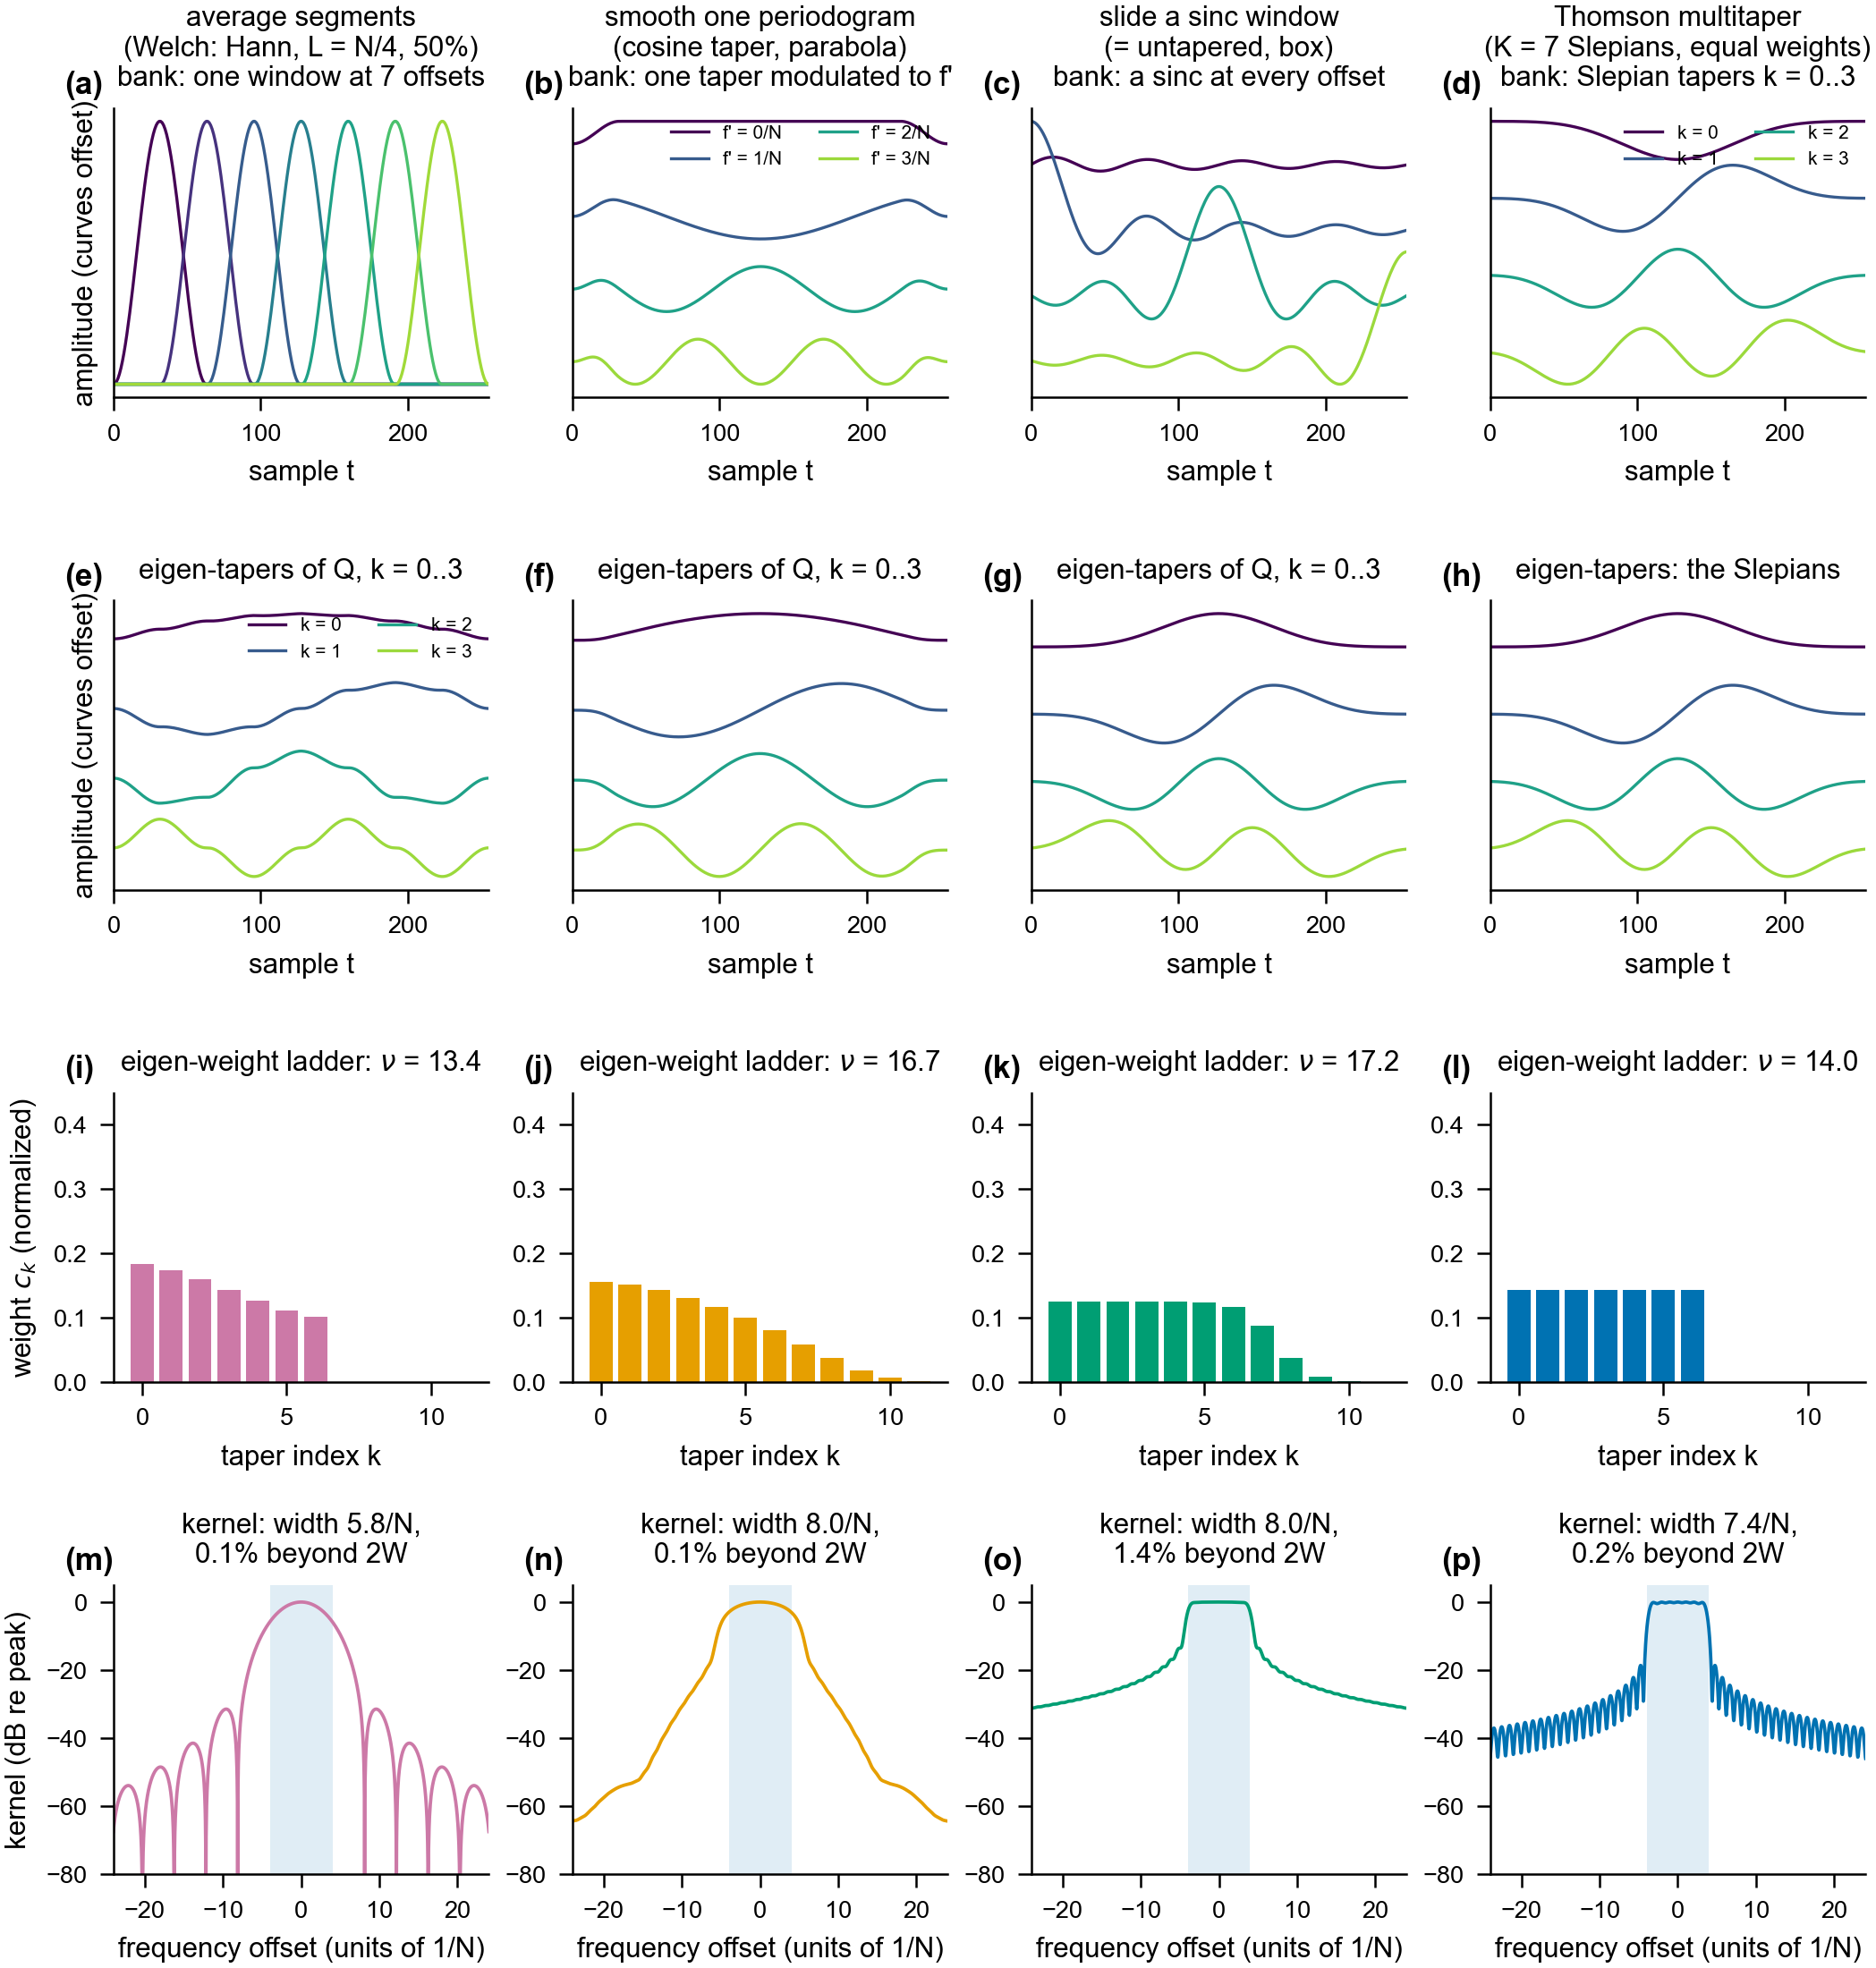
\includegraphics[width=\textwidth]{fig6_taper_banks_full.png}
\caption{\textbf{Fig.~\ref{fig:banks} in full.} Columns as in Fig.~\ref{fig:banks}; rows: the bank as constructed (a--d), the first four eigen-tapers of $Q$ (e--h; for the sliding sinc they are the Slepian sequences, and for Thomson's estimate, whose weights are equal, the Slepians are one of many orthonormal bases of the span), the eigen-weight ladder (i--l), and the kernel in dB relative to its peak with its half-power width and the fraction of its power beyond $2W$ (m--p; shading $|f|\le W$).}
\label{fig:banksfull}
\end{figure}

\begin{thebibliography}{99}
\bibitem{thomson1982} D.~J. Thomson, ``Spectrum estimation and harmonic analysis,'' \emph{Proc. IEEE}, vol.~70, no.~9, pp. 1055--1096, 1982. See Sec.~VIII, eq.~(8.3).
\bibitem{slepian1978} D.~Slepian, ``Prolate spheroidal wave functions, Fourier analysis, and uncertainty. V: The discrete case,'' \emph{Bell Syst. Tech. J.}, vol.~57, pp. 1371--1430, 1978.
\bibitem{babadi2014} B.~Babadi and E.~N. Brown, ``A review of multitaper spectral analysis,'' \emph{IEEE Trans. Biomed. Eng.}, vol.~61, no.~5, pp. 1555--1564, 2014.
\bibitem{prerau2017} M.~J. Prerau, R.~E. Brown, M.~T. Bianchi, J.~M. Ellenbogen, and P.~L. Purdon, ``Sleep neurophysiological dynamics through the lens of multitaper spectral analysis,'' \emph{Physiology}, vol.~32, no.~1, pp. 60--92, 2017.
\bibitem{kay1988} S.~M. Kay, \emph{Modern Spectral Estimation: Theory and Application}. Englewood Cliffs, NJ: Prentice-Hall, 1988.
\bibitem{bartlett1948} M.~S. Bartlett, ``Smoothing periodograms from time-series with continuous spectra,'' \emph{Nature}, vol.~161, pp. 686--687, 1948.
\bibitem{blackman1958} R.~B. Blackman and J.~W. Tukey, \emph{The Measurement of Power Spectra from the Point of View of Communications Engineering}. New York: Dover, 1958.
\bibitem{percival1993} D.~B. Percival and A.~T. Walden, \emph{Spectral Analysis for Physical Applications: Multitaper and Conventional Univariate Techniques}. Cambridge Univ. Press, 1993 (2nd ed., \emph{Spectral Analysis for Univariate Time Series}, 2020).
\bibitem{daniell1946} P.~J. Daniell, discussion of ``On the theoretical specification and sampling properties of autocorrelated time-series,'' \emph{J. Roy. Statist. Soc. Suppl.}, vol.~8, pp. 88--90, 1946.
\bibitem{riedel1995} K.~S. Riedel and A.~Sidorenko, ``Minimum bias multiple taper spectral estimation,'' \emph{IEEE Trans. Signal Process.}, vol.~43, no.~1, pp. 188--195, 1995.
\bibitem{riedel1994} K.~S. Riedel, A.~Sidorenko, and D.~J. Thomson, ``Spectral estimation of plasma fluctuations. I. Comparison of methods,'' \emph{Phys. Plasmas}, vol.~1, no.~3, pp. 485--500, 1994.
\bibitem{walden2000} A.~T. Walden, ``A unified view of multitaper multivariate spectral estimation,'' \emph{Biometrika}, vol.~87, no.~4, pp. 767--788, 2000.
\bibitem{abreu2017} L.~D. Abreu and J.~L. Romero, ``MSE estimates for multitaper spectral estimation and off-grid compressive sensing,'' \emph{IEEE Trans. Inf. Theory}, vol.~63, no.~12, pp. 7770--7776, 2017.
\bibitem{karnik2022} S.~Karnik, J.~Romberg, and M.~A. Davenport, ``Thomson's multitaper method revisited,'' \emph{IEEE Trans. Inf. Theory}, vol.~68, no.~7, pp. 4864--4891, 2022.
\bibitem{bronez1992} T.~P. Bronez, ``On the performance advantage of multitaper spectral analysis,'' \emph{IEEE Trans. Signal Process.}, vol.~40, no.~12, pp. 2941--2946, 1992.
\bibitem{hansson2012} M.~Hansson-Sandsten, ``A Welch method approximation of the Thomson multitaper spectrum estimator,'' in \emph{Proc. EUSIPCO}, Bucharest, 2012, pp. 440--444.
\bibitem{welch1967} P.~D. Welch, ``The use of fast Fourier transform for the estimation of power spectra: A method based on time averaging over short, modified periodograms,'' \emph{IEEE Trans. Audio Electroacoust.}, vol.~15, no.~2, pp. 70--73, 1967.
\bibitem{thomson1991} D.~J. Thomson and A.~D. Chave, ``Jackknifed error estimates for spectra, coherences, and transfer functions,'' in \emph{Advances in Spectrum Analysis and Array Processing}, vol.~1, S.~Haykin, Ed. Englewood Cliffs, NJ: Prentice-Hall, 1991, ch.~2, pp. 58--113.
\bibitem{bruns2004} A.~Bruns, ``Fourier-, Hilbert- and wavelet-based signal analysis: are they really different approaches?'' \emph{J. Neurosci. Methods}, vol.~137, no.~2, pp. 321--332, 2004.
\bibitem{wahba1980} G.~Wahba, ``Automatic smoothing of the log periodogram,'' \emph{J. Amer. Statist. Assoc.}, vol.~75, no.~369, pp. 122--132, 1980.
\bibitem{hurvich1985} C.~M. Hurvich, ``Data-driven choice of a spectrum estimate: extending the applicability of cross-validation methods,'' \emph{J. Amer. Statist. Assoc.}, vol.~80, no.~392, pp. 933--940, 1985.
\bibitem{haley2017} C.~L. Haley and M.~Anitescu, ``Optimal bandwidth for multitaper spectrum estimation,'' \emph{IEEE Signal Process. Lett.}, vol.~24, no.~11, pp. 1696--1700, 2017.
\bibitem{harris1978} F.~J. Harris, ``On the use of windows for harmonic analysis with the discrete Fourier transform,'' \emph{Proc. IEEE}, vol.~66, no.~1, pp. 51--83, 1978.
\bibitem{mitra1999} P.~P. Mitra and B.~Pesaran, ``Analysis of dynamic brain imaging data,'' \emph{Biophys. J.}, vol.~76, no.~2, pp. 691--708, 1999.
\bibitem{bokil2010} H.~Bokil, P.~Andrews, J.~E. Kulkarni, S.~Mehta, and P.~P. Mitra, ``Chronux: a platform for analyzing neural signals,'' \emph{J. Neurosci. Methods}, vol.~192, no.~1, pp. 146--151, 2010.
\bibitem{satterthwaite1946} F.~E. Satterthwaite, ``An approximate distribution of estimates of variance components,'' \emph{Biometrics Bull.}, vol.~2, no.~6, pp. 110--114, 1946.
\bibitem{nuttall1982} A.~H. Nuttall and G.~C. Carter, ``Spectral estimation using combined time and lag weighting,'' \emph{Proc. IEEE}, vol.~70, no.~9, pp. 1115--1125, 1982.
\end{thebibliography}

\end{document}
